
%%!TEX TS-program = latex

% [chama] $ pdflatex main.tex

% [local] $ ~/bin/  // bash scripts
% [local] $ la  // pdflatex -shell-escape main.tex
% [local] $ lae // la then open is TEMP explorer (Windows)
% [local] $ lax // la then open as main.pdf in explorer (Windows)


% --------------
% DOCUMENT CLASS
% --------------
% \documentclass[10pt,twoside,letterpaper,fleqn]{report}
\documentclass[11pt,letterpaper,fleqn]{report}
% \documentclass[12pt,letterpaper,fleqn]{article}
%\documentclass[12pt,a4paper,twoside,fleqn]{book}
% \documentclass[12pt,letterpaper,twoside,fleqn]{book}
% A4 paper measures 210 × 297 millimeters (8.27 × 11.69 inches).


% -------
% PACKAGE
% -------
% http://ctan.mirrors.hoobly.com/macros/latex/contrib/hyperref/doc/manual.pdf
\usepackage{hyperref}
\hypersetup{
  colorlinks=true, % instead of default boxed links, use color links
  linkcolor=blue, % instead of red default, use blue
  citecolor=blue, % instead of default green, use blue
  urlcolor=blue % instead of magenta default, use blue
} % close hyperref
%
\usepackage{framed} % for Hquote environment

\usepackage{amsmath} % needed for align of equations
\usepackage{amssymb}
\usepackage[toc,titletoc,header]{appendix}
\usepackage{datetime}  \renewcommand{\dateseparator}{-}
% \usepackage{epsfig}
% \usepackage{include/fancyheadings}
% \usepackage{fancyheadings}
\usepackage{fancyhdr}
\usepackage{multirow} 
\usepackage[percent]{overpic}  % \includegraphics 
% \usepackage{pifont} % required for dingbats
% \usepackage{psfrag}
%\usepackage[cleanup={.tex,.dvi,.ps,.log},process=all]{pstool}
%\usepackage{showframe} % bounding boxes on all LaTeX text areas
%\usepackage{subfigure} % requires \usepackage{epsfig} too
% \usepackage{cancel}
% 
% Lowercase fourth order tensors begin
% \usepackage{bbm}  % alternative to lowercase fourth order tensors
% \usepackage{bbold} % fourth order tensors from default serif to sans serif
% \usepackage{mathbbol}  % lowercase mathbb
% \usepackage[utf8]{inputenc}  % Unicode and TeX
% https://tex.stackexchange.com/questions/384265/how-to-use-mathbbol-only-for-greek-and-lowercase
% \usepackage[bbgreekl]{mathbbol} 
%   \DeclareSymbolFontAlphabet{\mathbbm}{bbold}
%   \DeclareSymbolFontAlphabet{\mathbb}{AMSb}
% % Lowercase fourth order tensors end
%
% \usepackage{enumitem}
%\usepackage[usenames, dvipsnames]{color}
%\definecolor{hg}{gray}{0.6} % Hovey gray
\usepackage[x11names,table]{xcolor}  % needed by ../book/h_math_ams.tex
% See color names at https://tex.stackexchange.com/questions/102777/does-anyone-have-a-newrgbcolorcolournamex-x-x-list
\usepackage[x11names]{xcolor}
\definecolor{hred}{rgb}{1,0,0}
\definecolor{hivory}{rgb}{1,1,0.94}
% \usepackage{tcolorbox}

\usepackage{minted}
% See minted documentation 
% http://mirrors.rit.edu/CTAN/macros/latex/contrib/minted/minted.pdf0
% $pdflatex -shell-escape main.tex

% \usepackage{showframe} % show/hide bounding boxes for all margins

% -------
% INCLUDE
% -------

%\include{include/Hformatams}
%\include{Hformatams}
% 2017-10-16 Too many version of Hformatams floating around, so 
% rename the format file used for the book to
% \include{h_math_ams}
% \include{hovey_styles}
% \input{../../material/doc/materials_colors}
% version 8 Oct 1998 
% Stanford University
% formerly Lausanne, Switzerland


% *-----------------------*
% | LaTeXING THE DOCUMENT |
% *-----------------------*--------------------------------------
%
% Run LaTeX on this file twice for proper section numbers.
% A '%' causes LaTeX to ignore remaining text on the line
% latex filename.tex
% dvips filename.dvi -o filename.ps
% ghostview filename.ps 
%
% *--------------------------------------------------------------


\newcommand{\ie}{{\em i.e., }}
\newcommand{\viz}{{\em viz.}}
\newcommand{\htable}{{\sc Table}}
\newcommand{\hfigure}{{\sc Figure}}

\newcommand{\hframe}[1]{{}^{\mathcal{#1}}\!}

% PLASTICITY - formulation
% ============
 \newcommand{\hstrain}{\varepsilon}
 \newcommand{\vhstrain}{\ve{\varepsilon}}
 \newcommand{\hstraindot}{\dot{\varepsilon}}
 \newcommand{\hstraine}{\varepsilon^{\mbox{\footnotesize e}}}
 \newcommand{\hstrainp}{\varepsilon^{\mbox{\footnotesize p}}}
 \newcommand{\hstrainpdot}{\dot{\varepsilon}^{\mbox{\footnotesize p}}}
 \newcommand{\gammadot}{\dot{\gamma}}
 \newcommand{\sign}{\mbox{sign}}
 \newcommand{\sigmadot}{\dot{\sigma}}  
 \newcommand{\vsigma}{\ve{\sigma}}  
 \newcommand{\vsigmavol}{\ve{\sigma}_{\tiny\mbox{VOL}}}
 \newcommand{\vsigmadev}{\ve{\sigma}_{\tiny\mbox{DEV}}}
 \newcommand{\Phidot}{\dot{\Phi}}
 \newcommand{\setequal}{\stackrel{\mbox{set}}{=}}
 \newcommand{\Cep}{C_{\mbox{\footnotesize ep}}}
 \newcommand{\Eep}{E_{\mbox{\footnotesize ep}}}
 \newcommand{\keq}{k_{\mbox{\footnotesize eq}}}
 \newcommand{\alphadot}{\dot{\alpha}}

% PLASTICITY - implementation
% ============
 \newcommand{\hstrainn}{\varepsilon_n}
 \newcommand{\hstrainen}{\varepsilon^{\mbox{\footnotesize e}}_{n}}
 \newcommand{\hstrainpn}{\varepsilon^{\mbox{\footnotesize p}}_{n}}
 \newcommand{\alphan}{\alpha_n}
 \newcommand{\gamman}{\gamma_n}
 \newcommand{\hstrainnp}{\varepsilon_{n+1}}
 \newcommand{\hstrainenp}{\varepsilon^{\mbox{\footnotesize e}}_{n+1}}
 \newcommand{\hstrainpnp}{\varepsilon^{\mbox{\footnotesize p}}_{n+1}}
 \newcommand{\hstrainpnpi}{\varepsilon^{\mbox{\footnotesize p}\;(i)}_{n+1}}
 \newcommand{\hstrainpnpip}{\varepsilon^{\mbox{\footnotesize p}\;(i+1)}_{n+1}}
 \newcommand{\hstrainptrnp}{\varepsilon^{\mbox{\footnotesize p tr}}_{n+1}}
 \newcommand{\alphanp}{\alpha_{n+1}}
 \newcommand{\alphanpi}{\alpha_{n+1}^{(i)}}
 \newcommand{\alphatrnp}{\alpha^{\mbox{\footnotesize tr}}_{n+1}}
 \newcommand{\alphanpip}{\alpha_{n+1}^{(i+1)}}
 \newcommand{\gammanp}{\gamma_{n+1}}
 \newcommand{\gammadotnp}{\dot{\gamma}_{n+1}} 

 \newcommand{\sigmatrnp}{\sigma^{\mbox{\footnotesize tr}}_{n+1}}
 \newcommand{\sigman}{\sigma_n}
 \newcommand{\sigmanp}{\sigma_{n+1}}

 \newcommand{\tn}{t_n}
 \newcommand{\tnp}{t_{n+1}}

 \newcommand{\Phinp}{\Phi_{n+1}}
 \newcommand{\Phidotnp}{\dot{\Phi}_{n+1}}
 \newcommand{\Phitrnp}{\Phi^{\mbox{\footnotesize tr}}_{n+1}}

% CIRCLED STATES
% ==============
\newcommand*\circled[1]{\tikz[baseline=(char.base)]{
            \node[shape=circle,draw,inner sep=2pt] (char) {#1};}}

% *--------------*
% | MATH SYMBOLS |
% *--------------*-----------------------------------------------
%
  \newcommand{\hcos}{\sf c}
  \newcommand{\hsin}{\sf s}
  \newcommand{\epi}{\mbox{epi }}
  \newcommand{\fa}{\forall \quad}
  \newcommand{\sotwo}{SO(2)}
  \newcommand{\sothree}{SO(3)}
% \newcommand {\angvel}[3]{{}^{#1}{#2}^{#3}}
% \newcommand{\implies}{\Rightarrow}
  \newcommand{\dirderiv}[1]{\mathbf{D}_{#1}}
  \newcommand{\abs}[1]{| \, #1 \, |}
  \newcommand{\innerproductmap}{\langle \, \cdot \, , \, \cdot \, \rangle}
  \newcommand{\innerproduct}[2]{\langle \, #1    \, , \, #2    \, \rangle}
  \newcommand{\normmap}{\parallel \, \cdot \, \parallel}
  \newcommand{\norm}[1]{\parallel~#1~\parallel}  
  \newcommand{\trace}{\mbox{tr}}
  \newcommand{\DEV}{\mbox{DEV}}
  \newcommand{\dev}{\mbox{dev}}
  \newcommand{\VOL}{\mbox{VOL}}
  \newcommand{\vol}{\mbox{vol}}
  \newcommand{\smDEV}{\mbox{\tiny DEV}}
  \newcommand{\smdev}{\mbox{\tiny dev}}
  \newcommand{\smVOL}{\mbox{\tiny VOL}}
  \newcommand{\smvol}{\mbox{\tiny vol}}
  \newcommand{\DEVoper}{\mbox{DEV}[\;\cdot\;]}
  \newcommand{\devoper}{\mbox{dev}[\;\cdot\;]}
  \newcommand{\ltwonorm}[1]{\parallel #1 \parallel_{_2}}
  \newcommand{\st}{\mbox{s.t. }}
  \newcommand{\pd}{\mbox{p.d. }}
  \newcommand{\defe}{\stackrel{\Delta}{=}}
  \newcommand{\dst}{\displaystyle} 
  \newcommand{\be}{\begin{equation}}
  \newcommand{\ee}{\end{equation}}
% \newcommand{\ve}[1]{\mathbf{#1}}
  \newcommand{\ve}[1]{\mbox{\boldmath $#1$}}
  \newcommand{\half}{\frac{1}{2}}


% the old diad that I commented out 5/24/96
% \newcommand{\di}[1]{\mathsf{#1}}
% this new one seems to work, helvetica under the file
% /usr/local/teTeX/texmf/fonts/tfm/adobe/helvetic/phvb8r.tfm
%  \font\gm=msym10  % <- this one doesn't work
  \font\gm=phvb8r   % this is helvetica font essentially
  \newcommand{\di}[1]{\hbox{\gm #1}}
  \font\idm=zptmcmrm
  \newcommand{\dii}{\hbox{\idm I}}
  \font\zaph=pzcmi8t
  \newcommand{\refframe}[1]{\hbox{\zaph #1}}

% \newcommand{\di}[1]{\hbox{\tenbfss #1}}
  \newcommand{\dib}[1]{\bf \mathsf{#1} }
%  \newcommand{\qed}{{\;\; \blacksquare} }
%
% *--------------------------------------------------------------

% THERMODYNAMICS
% ============
\newcommand{\svol}{\mathcal{V}}  % specific volume
\newcommand{\senergy}{\mathcal{E}} % specific total energy
\newcommand{\IE}{\mathcal{I}} % internal energy
\newcommand{\KE}{\mathcal{K}} % kinetic energy
\newcommand{\PE}{\mathcal{P}} % potential energy
\newcommand{\helmholtz}{\mathcal{F}} % Helmholtz free energy
\newcommand{\gibbs}{\mathcal{G}} % Gibbs free energy
\newcommand{\enthalpy}{\mathcal{H}} % enthalpy


% *--------------------------------------------------------------

% BIOMECHANICS
% ============
\newcommand{\Pmtar}{P_{\mbox{\tiny mtar}}}
\newcommand{\Pheel}{P_{\mbox{\tiny heel}}}


% VECTOR SPACE defined by Gurtin
% ==============================
\newcommand{\lin}{{\sc lin}}
\newcommand{\linplus}{{\sc lin}$^+$}
\newcommand{\sym}{{\sc sym}}
% skew is already defined, define as skw instead
% \newcommand{\skew}{{\sc skw}}
\newcommand{\skw}{{\sc skw}}
\newcommand{\psym}{{\sc psym}}
\newcommand{\orth}{{\sc orth}}
\newcommand{\orthplus}{{\sc orth}$^+$}
%
 
% VECTOR CALCULUS OPERATORS
% =========================

\newcommand{\Grad}{\ve{\nabla}_{\hspace{-1mm}\mbox{\tiny 0}}}
\newcommand{\grad}{\ve{\nabla}}
\newcommand{\gradX}{\ve{\nabla}}
\newcommand{\gradx}{\ve{\nabla}_{x}}
\renewcommand{\div}{\cdot}
\newcommand{\vdiv}{\ve{\cdot}}
\newcommand{\ddiv}{:}
\newcommand{\vddiv}{\ve{:}}
\newcommand{\union}{\cup}
\newcommand{\intersection}{\cap}

\newcommand{\DIV}{\mbox{DIV}}
%\newcommand{\div}{\mbox{div}}


% DINGBATS (CIRLED NUMBERS)
% (MUST ALSO HAVE \usepackage{pifont} IN HEADER
% =============================================
\newcommand{\circleone}{{\mbox{\small \ding{172}}}}
\newcommand{\circletwo}{{\mbox{\small \ding{173}}}}

% VECTOR ALPHABET
% ===============

\newcommand{\vA}{\ve{A}}
\newcommand{\va}{\ve{a}}
\newcommand{\Dva}{\Delta \va}
\newcommand{\vB}{\ve{B}}
\newcommand{\vb}{\ve{b}}
\newcommand{\vC}{\ve{C}}
\newcommand{\vCdot}{\dot{\ve{C}}}
\newcommand{\vCinv}{\ve{C}^{-1}}
\newcommand{\vc}{\ve{c}}
\newcommand{\vD}{\ve{D}}
\newcommand{\vd}{\ve{d}}
\newcommand{\Dvd}{\Delta \vd}
\newcommand{\vE}{\ve{E}}
\newcommand{\vEdot}{\dot{\ve{E}}}
\newcommand{\vF}{\ve{F}}
\newcommand{\vFdot}{\dot{\ve{F}}}
\newcommand{\vf}{\ve{f}}
\newcommand{\vG}{\ve{G}}
\newcommand{\vg}{\ve{g}}
\newcommand{\gdot}{\dot{g}}
\newcommand{\vH}{\ve{H}}
\newcommand{\vh}{\ve{h}}
\newcommand{\vI}{\ve{I}}
\newcommand{\vid}{\ve{1}}
\newcommand{\vJ}{\ve{J}}
\newcommand{\vK}{\ve{K}}
%\newcommand{\vKe}{\ve{K}^{\mbox{\tiny e}}} % already defined
\newcommand{\vL}{\ve{L}}
\newcommand{\vl}{\ve{l}}
\newcommand{\vM}{\ve{M}}
\newcommand{\vN}{\ve{N}}
\newcommand{\vn}{\ve{n}}
\newcommand{\vnhat}{\hat{\ve{n}}}
\newcommand{\vO}{\ve{O}}
\newcommand{\vP}{\ve{P}}
\newcommand{\vp}{\ve{p}}
\newcommand{\vPelas}{\ve{P}^{\mbox{\tiny elas}}}
\newcommand{\vPvisc}{\ve{P}^{\mbox{\tiny visc}}}
\newcommand{\vQ}{\ve{Q}}
\newcommand{\vq}{\ve{q}}
\newcommand{\vqdot}{\dot{\ve{q}}}
\newcommand{\vqddot}{\ddot{\ve{q}}}
\newcommand{\vR}{\ve{R}}
\newcommand{\vr}{\ve{r}}
\newcommand{\vrhat}{\hat{\ve{r}}}
\newcommand{\vS}{\ve{S}}
\newcommand{\vSelas}{\ve{S}^{\mbox{\tiny elas}}} 
\newcommand{\vSvisc}{\ve{S}^{\mbox{\tiny visc}}}
\newcommand{\vs}{\ve{s}}
\newcommand{\vsdot}{\dot{\ve{s}}}
\newcommand{\vsddot}{\ddot{\ve{s}}}
\newcommand{\vshat}{\hat{\ve{s}}}
\newcommand{\vT}{\ve{T}}
\newcommand{\vTbar}{\bar{\ve{T}}}
\newcommand{\vThat}{\hat{\ve{T}}}
\newcommand{\vTT}{\vT_{\mbox{\tiny T}}}
\newcommand{\vt}{\ve{t}}
\newcommand{\vthat}{\hat{\ve{t}}}
\newcommand{\vU}{\ve{U}}
\newcommand{\vUbar}{\bar{\ve{U}}}
\newcommand{\vUdot}{\dot{\ve{U}}}
\newcommand{\vUddot}{\ddot{\ve{U}}}
\newcommand{\vu}{\ve{u}}
\newcommand{\DvU}{\Delta \vU}
\newcommand{\vV}{\ve{V}}
\newcommand{\vv}{\ve{v}}
\newcommand{\Dvv}{\Delta \vv}
\newcommand{\vW}{\ve{W}}
\newcommand{\vw}{\ve{w}}
\newcommand{\vX}{\ve{X}}
\newcommand{\vx}{\ve{x}}
\newcommand{\vxhat}{\hat{\ve{x}}}
\newcommand{\vY}{\ve{Y}}
\newcommand{\vy}{\ve{y}}
\newcommand{\vyhat}{\hat{\ve{y}}}
\newcommand{\vZ}{\ve{Z}}
\newcommand{\vz}{\ve{z}}

% VECTOR NUMBERS
% ==============
  \newcommand{\vzero}{\ve{0}}

% BLACKBOARD ALPHABET
% ===================
  \newcommand{\dist}{\mathbb{D}}
  \newcommand{\proj}{\mathbb{P}}
  \newcommand{\projT}{\proj_{\mbox{\tiny T}}}
  \newcommand{\interval}{\mathbb{T}}

% VECTOR GREEK ALPHABET
% =====================
  \newcommand{\vDelta}{\ve{\Delta}}
  \newcommand{\vdelta}{\ve{\delta}}
  \newcommand{\vkappa}{\ve{\kappa}}
  \newcommand{\vLambda}{\ve{\Lambda}}
  \newcommand{\vlambda}{\ve{\lambda}}
  \newcommand{\vphi}{\ve{\phi}}
  \newcommand{\vvarphi}{\ve{\varphi}}
  \newcommand{\vvarphidot}{\dot{\ve{\varphi}}}
  \newcommand{\vvarphiddot}{\ddot{\ve{\varphi}}}
  \newcommand{\vxi}{\ve{\xi}}
  \newcommand{\vthetahat}{\hat{\ve{\theta}}}
  \newcommand{\vtau}{\ve{\tau}}

% CALIGRAPHY ALPHABET
% ===================
  \newcommand{\cA}{\mathcal{A}}
  \newcommand{\cB}{\mathcal{B}}
  \newcommand{\cC}{\mathcal{C}}
  \newcommand{\cD}{\mathcal{D}}
  \newcommand{\cE}{\mathcal{E}}
  \newcommand{\cF}{\mathcal{F}}
  \newcommand{\cG}{\mathcal{G}}
  \newcommand{\cI}{\mathcal{I}}
  \newcommand{\cJ}{\mathcal{J}}
  \newcommand{\cK}{\mathcal{K}}
  \newcommand{\cL}{\mathcal{L}}
  \newcommand{\cO}{\mathcal{O}}
  \newcommand{\cP}{\mathcal{P}}
  \newcommand{\cQ}{\mathcal{Q}}
  \newcommand{\cR}{\mathcal{R}}  
  \newcommand{\cS}{\mathcal{S}}
  \newcommand{\cV}{\mathcal{V}}
  \newcommand{\cW}{\mathcal{W}}


% ENERGY ALPHABET
% ===============
  \newcommand{\Vext}{V^{\mbox{\tiny ext}}}
  \newcommand{\Vint}{V^{\mbox{\tiny int}}}

% Second and Fourth Order Tensor ALPHABET
% ========================================
%\newcommand{\tC}{\mathbb{C}}
%\newcommand{\tI}{\mathbb{I}}
%\newcommand{\tV}{\mathbb{V}}
% fourth-order tensor 
\newcommand{\fotA}{\mathbb{A}}
%\newcommand{\fota}{{\rm a\kern-0.19em \tiny |}}
\newcommand{\fota}{\mathbb{a}}
\newcommand{\fotC}{\mathbb{C}}

\newcommand{\transpose}{^{\mbox{\scriptsize \sffamily T}}}

\newcommand{\tA}{\mathsf A}
%\newcommand{\ta}{\mbox{\sffamily a}}
%\newcommand{\tb}{\mbox{\sffamily b}}
%\newcommand{\tC}{\mbox{\sffamily C}}
%\newcommand{\tE}{\mbox{\sffamily E}}
%\newcommand{\te}{\mbox{\sffamily e}}
%\newcommand{\tF}{\mbox{\sffamily F}}
%\newcommand{\tI}{\mbox{\rmfamily I}}
%\newcommand{\tM}{\mbox{\sffamily M}}
%\newcommand{\tP}{\mbox{\sffamily P}}
%\newcommand{\tQ}{\mbox{\sffamily Q}}
%\newcommand{\tR}{\mbox{\sffamily R}}
%\newcommand{\ts}{\mbox{\sffamily s}}
%\newcommand{\tV}{\mbox{\sffamily V}}
\newcommand{\ta}{\mathsf a}
\newcommand{\tb}{\mathsf b}
\newcommand{\tC}{\mathsf C}
\newcommand{\tE}{\mathsf E}
\newcommand{\te}{\mathsf e}
\newcommand{\tF}{\mathsf F}
\newcommand{\tI}{\mathsf I}
\newcommand{\tM}{\mathsf M}
\newcommand{\tP}{\mathsf P}
\newcommand{\tQ}{\mathsf Q}
\newcommand{\tR}{\mathsf R}
\newcommand{\ts}{\mathsf s}
\newcommand{\tV}{\mathsf V}

\newcommand{\tAbold}{\mbox{\sffamily\bfseries A}}
\newcommand{\tabold}{\mbox{\sffamily\bfseries a}}
\newcommand{\tbbold}{\mbox{\sffamily\bfseries b}}
\newcommand{\tCbold}{\mbox{\sffamily\bfseries C}}
\newcommand{\tebold}{\mbox{\sffamily\bfseries e}}
\newcommand{\tEbold}{\mbox{\sffamily\bfseries E}}
\newcommand{\tFbold}{\mbox{\sffamily\bfseries F}}
\newcommand{\tIbold}{\mbox{\rmfamily\bfseries I}}
\newcommand{\tMbold}{\mbox{\sffamily\bfseries M}}
\newcommand{\tPbold}{\mbox{\sffamily\bfseries P}}
\newcommand{\tQbold}{\mbox{\sffamily\bfseries Q}}
\newcommand{\tRbold}{\mbox{\sffamily\bfseries R}}
\newcommand{\tSbold}{\mbox{\sffamily\bfseries S}}
\newcommand{\tsbold}{\mbox{\sffamily\bfseries s}}
\newcommand{\tUbold}{\mbox{\sffamily\bfseries U}}
\newcommand{\tVbold}{\mbox{\sffamily\bfseries V}}

\newcommand{\tICinv}{\tIbold_{C^{-1}}}

\newcommand{\tc}{\mbox{\sffamily\large c}}
\newcommand{\ti}{\mbox{\rmfamily\large i}}
\newcommand{\tv}{\mbox{\sffamily\large v}}

\newcommand{\tcbold}{\mbox{\sffamily\bfseries\large c}}
\newcommand{\tibold}{\mbox{\rmfamily\bfseries\large i}}
\newcommand{\tvbold}{\mbox{\sffamily\bfseries\large v}}

%\newcommand{\assembly}{\overset{n_{el}}{\underset{e=1}{
%  \mbox{ \sffamily\bfseries \large A } }}}

% Tensor INVARIANTS
% =================
\newcommand{\invCone}{\mbox{\rmfamily I}_C}
\newcommand{\invCtwo}{\mbox{\rmfamily II}_C}
\newcommand{\invCthree}{\mbox{\rmfamily III}_C}

% RIGID BODY  NOTATION
% ====================
% plain variable
\newcommand{\vucm}{\overset{*}{\ve{u}}}
\newcommand{\vvcm}{\overset{*}{\ve{v}}}
\newcommand{\vacm}{\overset{*}{\ve{a}}}
\newcommand{\vXcm}{\overset{*}{\ve{X}}}
\newcommand{\Xcm}{\overset{*}{X}}
\newcommand{\vxcm}{\overset{*}{\ve{x}}}
\newcommand{\vvarphicm}{\overset{*}{\ve{\varphi}}}
\newcommand{\vtheta}{\ve{\theta}}
\newcommand{\thetadot}{\dot{\theta}}
\newcommand{\vthetadot}{\dot{\ve{\theta}}}
\newcommand{\vthetaddot}{\ddot{\ve{\theta}}}
\newcommand{\vomega}{\ve{\omega}}
\newcommand{\vomegahat}{\widehat{\ve{\omega}}}
\newcommand{\vpsi}{\ve{\psi}}
\newcommand{\psidot}{\dot{\psi}}
\newcommand{\vpsidot}{\dot{\ve{\psi}}}
\newcommand{\valpha}{\ve{\alpha}}
\newcommand{\vpi}{\ve{\pi}}

\newcommand{\vvCinB}{}

%  at time n
\newcommand{\vucmn}{\overset{*}{\ve{u}}_n}
\newcommand{\vvcmn}{\overset{*}{\ve{v}}_n}
\newcommand{\vacmn}{\overset{*}{\ve{a}}_n}
\newcommand{\vXcmn}{\overset{*}{\ve{X}}_n}
\newcommand{\vxcmn}{\overset{*}{\ve{x}}_n}
\newcommand{\vvarphicmn}{\overset{*}{\ve{\varphi}}_n}
\newcommand{\vthetan}{\ve{\theta}_n}
\newcommand{\vthetadotn}{\dot{\ve{\theta}}_n}
\newcommand{\vthetaddotn}{\ddot{\ve{\theta}}_n}
\newcommand{\vomegan}{\ve{\omega}_n}
\newcommand{\valphan}{\ve{\alpha}_n}

% at time n+1
\newcommand{\vucmnp}{\overset{*}{\ve{u}}_{n+1}}
\newcommand{\vvcmnp}{\overset{*}{\ve{v}}_{n+1}}
\newcommand{\vacmnp}{\overset{*}{\ve{a}}_{n+1}}
\newcommand{\vXcmnp}{\overset{*}{\ve{X}}_{n+1}}
\newcommand{\vxcmnp}{\overset{*}{\ve{x}}_{n+1}}
\newcommand{\vvarphicmnp}{\overset{*}{\ve{\varphi}}_{n+1}}
\newcommand{\vthetanp}{\ve{\theta}_{n+1}}
\newcommand{\vthetadotnp}{\dot{\ve{\theta}}_{n+1}}
\newcommand{\vthetaddotnp}{\ddot{\ve{\theta}}_{n+1}}
\newcommand{\vomeganp}{\ve{\omega}_{n+1}}
\newcommand{\valphanp}{\ve{\alpha}_{n+1}}

% at time n+1 iteration i
\newcommand{\vucmnpi}{\overset{*}{\ve{u}}_{n+1}^{(i)}}
\newcommand{\vvcmnpi}{\overset{*}{\ve{v}}_{n+1}^{(i)}}
\newcommand{\vacmnpi}{\overset{*}{\ve{a}}_{n+1}^{(i)}}
\newcommand{\vXcmnpi}{\overset{*}{\ve{X}}_{n+1}^{(i)}}
\newcommand{\vxcmnpi}{\overset{*}{\ve{x}}_{n+1}^{(i)}}
\newcommand{\vvarphicmnpi}{\overset{*}{\ve{\varphi}}_{n+1}^{(i)}}
\newcommand{\Dvucmnpi}{\Delta \overset{*}{\ve{u}}_{n+1}^{(i)}}
\newcommand{\vthetanpi}{\ve{\theta}_{n+1}^{(i)}}
\newcommand{\vthetadotnpi}{\dot{\ve{\theta}}_{n+1}^{(i)}}
\newcommand{\vthetaddotnpi}{\ddot{\ve{\theta}}_{n+1}^{(i)}}
\newcommand{\vomeganpi}{\ve{\omega}_{n+1}^{(i)}}
\newcommand{\valphanpi}{\ve{\alpha}_{n+1}^{(i)}}


% at time n+1 iteration i+1
\newcommand{\vucmnpip}{\overset{*}{\ve{u}}_{n+1}^{(i+1)}}
\newcommand{\vvcmnpip}{\overset{*}{\ve{v}}_{n+1}^{(i+1)}}
\newcommand{\vacmnpip}{\overset{*}{\ve{a}}_{n+1}^{(i+1)}}
\newcommand{\vXcmnpip}{\overset{*}{\ve{X}}_{n+1}^{(i+1)}}
\newcommand{\vxcmnpip}{\overset{*}{\ve{x}}_{n+1}^{(i+1)}}
\newcommand{\vvarphicmnpip}{\overset{*}{\ve{\varphi}}_{n+1}^{(i+1)}}
\newcommand{\vthetanpip}{\ve{\theta}_{n+1}^{(i+1)}}
\newcommand{\vthetadotnpip}{\dot{\ve{\theta}}_{n+1}^{(i+1)}}
\newcommand{\vthetaddotnpip}{\ddot{\ve{\theta}}_{n+1}^{(i+1)}}
\newcommand{\vomeganpip}{\ve{\omega}_{n+1}^{(i+1)}}
\newcommand{\valphanpip}{\ve{\alpha}_{n+1}^{(i+1)}}


% volumes and other geometry
\newcommand{\OmegaR}{\Omega_R}
\newcommand{\intOmegaR}{\int_{\Omega_R}}
\newcommand{\intOmegaRe}{\int_{\Omega_R^e}}
\newcommand{\OmegaOne}{\Omega_1}
\newcommand{\OmegaTwo}{\Omega_2}

% masses and ineritas
%\newcommand{\inertia}{{\mbox{\rmfamily\bfseries I}}}
%\newcommand{\inertiaJ}{{\mbox{\rmfamily\bfseries J}}}
\newcommand{\inertia}{\mathbb I}
\newcommand{\inertiaJ}{\mathbb J}

% inertia at time n
\newcommand{\inertian}{{\mathbb I}_n}
\newcommand{\inertiaJn}{{\mathbb J}_n}

% END RIGID BODY NOTATION
% =======================


% *---------------*
% | BASIS VECTORS |
% *---------------*----------------------------------------------

%\newcommand{\veaa}{\hat{\ve{e}}_{01}}
%\newcommand{\veab}{\hat{\ve{e}}_{02}}
%\newcommand{\veac}{\hat{\ve{e}}_{03}}
%\newcommand{\veaa}{^{A}\hat{\ve{e}}_{1}}
%\newcommand{\veab}{^{A}\hat{\ve{e}}_{2}}
%\newcommand{\veac}{^{A}\hat{\ve{e}}_{3}}
%\newcommand{\veaa}{\hat{\ve{a}}_{1}}
%\newcommand{\veab}{\hat{\ve{a}}_{2}}
%\newcommand{\veac}{\hat{\ve{a}}_{3}}
\newcommand{\vea}{\hat{\ve{\sf{a}}}}
\newcommand{\veaa}{\hat{\ve{\sf{a}}}_1}
\newcommand{\veab}{\hat{\ve{\sf{a}}}_2}
\newcommand{\veac}{\hat{\ve{\sf{a}}}_3}
%
%\newcommand{\veba}{\hat{\ve{e}}_{11}}
%\newcommand{\vebb}{\hat{\ve{e}}_{12}}
%\newcommand{\vebc}{\hat{\ve{e}}_{13}}
%\newcommand{\veba}{\hat{\ve{b}}_{1}}
%\newcommand{\vebb}{\hat{\ve{b}}_{2}}
%\newcommand{\vebc}{\hat{\ve{b}}_{3}}
\newcommand{\veb}{\hat{\ve{\sf{b}}}}
\newcommand{\veba}{\hat{\ve{\sf{b}}}_1}
\newcommand{\vebb}{\hat{\ve{\sf{b}}}_2}
\newcommand{\vebc}{\hat{\ve{\sf{b}}}_3}
%

%\newcommand{\veca}{\hat{\ve{e}}_{21}}
%\newcommand{\vecb}{\hat{\ve{e}}_{22}}
%\newcommand{\vecc}{\hat{\ve{e}}_{23}}
\newcommand{\veca}{\hat{\ve{c}}_{1}}
\newcommand{\vecb}{\hat{\ve{c}}_{2}}
\newcommand{\vecc}{\hat{\ve{c}}_{3}}
%%
\newcommand{\veda}{\hat{\ve{e}}_{31}}
\newcommand{\vedb}{\hat{\ve{e}}_{32}}
\newcommand{\vedc}{\hat{\ve{e}}_{33}}
%
\newcommand{\veea}{\hat{\ve{e}}_{41}}
\newcommand{\veeb}{\hat{\ve{e}}_{42}}
\newcommand{\veec}{\hat{\ve{e}}_{43}}
%
%\newcommand{\veca}{\hat{\ve{e}}_{\cC1}}
%\newcommand{\vecb}{\hat{\ve{e}}_{\cC2}}
%\newcommand{\vecc}{\hat{\ve{e}}_{\cC3}}
%
%\newcommand{\vefa}{\hat{\ve{e}}_{\cF1}}
%\newcommand{\vefb}{\hat{\ve{e}}_{\cF2}}
%\newcommand{\vefc}{\hat{\ve{e}}_{\cF3}}
\newcommand{\vefa}{\hat{\ve{\sf{f}}}_1}
\newcommand{\vefb}{\hat{\ve{\sf{f}}}_2}
\newcommand{\vefc}{\hat{\ve{\sf{f}}}_3}



%
\newcommand{\veva}{\hat{\ve{e}}_{\cV1}}
\newcommand{\vevb}{\hat{\ve{e}}_{\cV2}}
\newcommand{\vevc}{\hat{\ve{e}}_{\cV3}}


\newcommand{\veihat}{\hat{\ve{\sf{i}}}}
\newcommand{\vejhat}{\hat{\ve{\sf{j}}}}
\newcommand{\vekhat}{\hat{\ve{\sf{k}}}}

\newcommand{\veEihat}{\hat{\ve{E}}_I}
\newcommand{\veEjhat}{\hat{\ve{E}}_J}
\newcommand{\veEkhat}{\hat{\ve{E}}_K}
\newcommand{\veElhat}{\hat{\ve{E}}_L}

\newcommand{\veeihat}{\hat{\ve{e}}_i}
\newcommand{\veejhat}{\hat{\ve{e}}_j}
\newcommand{\veekhat}{\hat{\ve{e}}_k}
\newcommand{\veelhat}{\hat{\ve{e}}_l}

\newcommand{\veeonehat}{\hat{\ve{\sf{e}}}_1}
\newcommand{\veetwohat}{\hat{\ve{\sf{e}}}_2}
\newcommand{\veethreehat}{\hat{\ve{\sf{e}}}_3}


% FEA OPERATOR NOTATION
% =====================
\newcommand{\Moper}{\mathcal{M}(\cdot,\cdot)}
\newcommand{\Meoper}{\mathcal{M}(\cdot,\cdot)^e}
\newcommand{\Noper}{\mathcal{N}(\cdot;\cdot,\cdot)}
\newcommand{\Neoper}{\mathcal{N}(\cdot;\cdot,\cdot)^e}
\newcommand{\Boper}{(\cdot,\cdot)}
\newcommand{\Beoper}{(\cdot,\cdot)^e}
\newcommand{\Toper}{(\cdot,\cdot)_{\Gamma_H}}
\newcommand{\Teoper}{(\cdot,\cdot)^e_{\Gamma_H}}

% FEA INTEGERS
% ============
\newcommand{\nel}{n_{\mbox{\tiny el}}}
\newcommand{\nen}{n_{\mbox{\tiny en}}}
\newcommand{\nsd}{n_{\mbox{\tiny sd}}}
%\newcommand{\neq}{n_{\mbox{\tiny eq}}}
\newcommand{\numeq}{n_{\mbox{\tiny eq}}}
\newcommand{\nts}{n_{\mbox{\tiny ts}}}
\newcommand{\naf}{n_{\mbox{\tiny af}}}
\newcommand{\nam}{n_{\mbox{\tiny am}}}
\newcommand{\nat}{n_{\mbox{\tiny at}}}

\newcommand{\GDYN}{G_{\mbox{\tiny DYN}}}

% SHAPE FUNCTION TRIAL FUNCTION
% =============================

\newcommand{\Uh}{U^h}
\newcommand{\Uhi}{U^h_i}
\newcommand{\vUh}{\ve{U}^h}
\newcommand{\vUt}{\ve{U}_t}
\newcommand{\vUhdot}{\dot{\ve{U}}^h}

\newcommand{\Wh}{W^h}
\newcommand{\Whi}{W^h_i}
\newcommand{\vWh}{\ve{W}^h}

\newcommand{\vTt}{\ve{T}_t}

\newcommand{\Kh}{K^h}
\newcommand{\Khi}{K^h_i}
\newcommand{\vKh}{\ve{K}^h}

\newcommand{\vcK}{\ve{\mathcal{K}}}
\newcommand{\vcKh}{\ve{\mathcal{K}}^h}
\newcommand{\vcV}{\ve{\mathcal{V}}}
\newcommand{\vcVh}{\ve{\mathcal{V}}^h}
\newcommand{\vcW}{\ve{\mathcal{W}}}
\newcommand{\vcWh}{\ve{\mathcal{W}}^h}
\newcommand{\vcS}{\ve{\mathcal{S}}}
\newcommand{\vcSh}{\ve{\mathcal{S}}^h}
\newcommand{\vcC}{\ve{\mathcal{C}}}

% RIGID BODY MASS CENTERS
% =======================
\newcommand{\Bstar}{B^{*}}

% INTEGRATION SYMBOLS
% ===================

\newcommand{\Omegae}{\Omega^e}

\newcommand{\intBox}{\int_{\Box}}

\newcommand{\intOmega}{\int_{\Omega}}
\newcommand{\intOmegae}{\int_{\Omega^e}}
\newcommand{\intomega}{\int_{\omega}}
\newcommand{\intomegae}{\int_{\omega^e}}


\newcommand{\intGamma}{\int_{\Gamma}}
\newcommand{\intgamma}{\int_{\gamma}}
\newcommand{\intGammaH}{\int_{\Gamma_H}}
\newcommand{\intGammaT}{\int_{\Gamma_T}}
\newcommand{\intGammaU}{\int_{\Gamma_U}}
\newcommand{\intGammaC}{\int_{\Gamma_C}}
\newcommand{\intGammaHe}{\int_{\Gamma^e_H}}
\newcommand{\intgammah}{\int_{\gamma_h}}

\newcommand{\intOmegaalpha}{\int_{\Omega^{(\alpha)}}}
\newcommand{\intGammaalpha}{\int_{\Gamma^{(\alpha)}}}
\newcommand{\intGammaone}{\int_{\Gamma^{(1)}}}
\newcommand{\intGammatwo}{\int_{\Gamma^{(2)}}}
\newcommand{\intGammaTalpha}{\int_{\Gamma_T^{(\alpha)}}}
\newcommand{\intGammaCalpha}{\int_{\Gamma_C^{(\alpha)}}}
\newcommand{\intGammaCone}{\int_{\Gamma_C^{(1)}}}
\newcommand{\intGammaCtwo}{\int_{\Gamma_C^{(2)}}}

\newcommand{\GammaH}{\Gamma_{H}}


\newcommand{\dOmega}{\; d\Omega}
\newcommand{\domega}{\; d\omega}
\newcommand{\dGamma}{\; d\Gamma}
\newcommand{\dgamma}{\; d\gamma}
\newcommand{\dGammaC}{\; d\Gamma_C}
\newcommand{\dBox}{\; d\;\Box}
\newcommand{\dOmegaalpha}{\; d\Omega^{(\alpha)}} 
\newcommand{\dGammaalpha}{\; d\Gamma^{(\alpha)}}

\newcommand{\deltae}{\delta^{\mbox{\tiny e}}}
\newcommand{\vdeltae}{\ve{\delta}^{\mbox{\tiny e}}}
\newcommand{\Deltae}{\Delta^{\mbox{\tiny e}}}
\newcommand{\vDeltae}{\ve{\Delta}^{\mbox{\tiny e}}}
 
\newcommand{\sone}{^{(1)}}
\newcommand{\stwo}{^{(2)}}
\newcommand{\sa}{^{(\alpha)}}


% *-----------------------------*
% | STRUCTURAL DYNAMICS SYMBOLS |
% *-----------------------------*--------------------------------

%\newcommand{\vd}{\ve{d}}
%\newcommand{\vv}{\ve{v}}
%\newcommand{\va}{\ve{a}}

\newcommand{\vdn}{\ve{d}_{n}}
\newcommand{\vun}{\ve{u}_{n}}
\newcommand{\vue}{\ve{u}^{\mbox{\tiny e}}}
\newcommand{\vUn}{\ve{U}_{n}}
\newcommand{\vvn}{\ve{v}_{n}}
\newcommand{\van}{\ve{a}_{n}}

\newcommand{\vdnp}{\ve{d}_{n+1}}
\newcommand{\vunp}{\ve{u}_{n+1}}
\newcommand{\vUnp}{\ve{U}_{n+1}}
\newcommand{\vvnp}{\ve{v}_{n+1}}
\newcommand{\vanp}{\ve{a}_{n+1}}

\newcommand{\vdnpa}{\ve{d}_{n+\alpha}}
\newcommand{\vunpa}{\ve{u}_{n+\alpha}}
\newcommand{\vUnpa}{\ve{U}_{n+\alpha}}
\newcommand{\vvnpa}{\ve{v}_{n+\alpha}}
\newcommand{\vVnpa}{\ve{V}_{n+\alpha}}
\newcommand{\vanpa}{\ve{a}_{n+\alpha}}
\newcommand{\vAnpa}{\ve{A}_{n+\alpha}}


\newcommand{\vdnm}{\ve{d}_{n-1}}
\newcommand{\vunm}{\ve{u}_{n-1}}
\newcommand{\vvnm}{\ve{v}_{n-1}}
\newcommand{\vanm}{\ve{a}_{n-1}}

\newcommand{\vdni}{\ve{d}_{n}^{(i)}}
\newcommand{\vuni}{\ve{u}_{n}^{(i)}}
\newcommand{\vUni}{\ve{U}_{n}^{(i)}}
\newcommand{\vvni}{\ve{v}_{n}^{(i)}}
\newcommand{\vani}{\ve{a}_{n}^{(i)}}

\newcommand{\vdnpi}{\ve{d}_{n+1}^{(i)}}
\newcommand{\vunpi}{\ve{u}_{n+1}^{(i)}}
\newcommand{\vUnpi}{\ve{U}_{n+1}^{(i)}}
\newcommand{\vvnpi}{\ve{v}_{n+1}^{(i)}}
\newcommand{\vanpi}{\ve{a}_{n+1}^{(i)}}

\newcommand{\vdnpip}{\ve{d}_{n+1}^{(i+1)}}
\newcommand{\vunpip}{\ve{u}_{n+1}^{(i+1)}}
\newcommand{\vVnpip}{\ve{U}_{n+1}^{(i+1)}}
\newcommand{\vvnpip}{\ve{v}_{n+1}^{(i+1)}}
\newcommand{\vanpip}{\ve{a}_{n+1}^{(i+1)}}

%\newcommand{\vM}{\ve{M}}
\newcommand{\vMs}{\ve{M}^{*}}
\newcommand{\vMnpi}{\vM_{n+1}^{(i)}}
%\newcommand{\vC}{\ve{C}}
\newcommand{\vDnpi}{\vD_{n+1}^{(i)}}
%\newcommand{\vK}{\ve{K}}
\newcommand{\vKe}{\ve{K}^{\mbox{\tiny e}}}
\newcommand{\vKd}{\ve{K}(\ve{d})}
\newcommand{\vKnpi}{\ve{K}_{n+1}^{(i)}}
%\newcommand{\vN}{\ve{N}}
\newcommand{\vNd}{\ve{N}(\ve{d})}
\newcommand{\vNdn}{\ve{N}(\ve{d}_{n})}
\newcommand{\vNdnp}{\ve{N}(\ve{d}_{n+1})}
\newcommand{\vNdnpi}{\ve{N}(\ve{d}_{n+1}^{(i)})}
\newcommand{\vNdnpip}{\ve{N}(\ve{d}_{n+1}^{(i+1)})}

\newcommand{\vVn}{\ve{V}_{n}}
\newcommand{\vVnp}{\ve{V}_{n+1}}

\newcommand{\vvarphin}{\ve{\varphi}_{n}}
\newcommand{\vvarphinp}{\ve{\varphi}_{n+1}}
\newcommand{\vvarphinpa}{\ve{\varphi}_{n+\alpha}}


\newcommand{\vFint}{\ve{F}^{\mbox{\tiny int}}}
\newcommand{\vFinte}{\ve{F}^{\mbox{\tiny int,e}}}
\newcommand{\vFintvisc}{\ve{F}^{\mbox{\tiny int,visc}}}
\newcommand{\vFintelas}{\ve{F}^{\mbox{\tiny int,elas}}}
\newcommand{\vFiner}{\ve{F}^{\mbox{\tiny iner}}}
\newcommand{\vFext}{\ve{F}^{\mbox{\tiny ext}}}
\newcommand{\vFexte}{\ve{F}^{\mbox{\tiny ext,e}}}
\newcommand{\vFextn}{\vFext(t_{n})}
\newcommand{\vFextnp}{\vFext(t_{n+1})}
\newcommand{\vFextnpa}{\vFext(t_{n+1+\alpha})}
\newcommand{\vFapp}{\ve{F}^{\mbox{\tiny app}}}

\newcommand{\vMext}{\ve{M}^{ext}}
\newcommand{\vMapp}{\ve{M}^{\mbox{\tiny app}}}
\newcommand{\vTapp}{\ve{T}^{\mbox{\tiny app}}}



\newcommand{\vfint}{\ve{f}^{\mbox{\tiny int}}}
\newcommand{\vfext}{\ve{f}^{\mbox{\tiny ext}}}
\newcommand{\vfextn}{\vfext(t_{n})}
\newcommand{\vfextnp}{\vfext(t_{n+1})}
\newcommand{\vfextnpa}{\vfext(t_{n+1+\alpha})}

\newcommand{\vddd}{\ddot{\ve{d}}}
\newcommand{\vdd}{\dot{\ve{d}}}
% \newcommand{\vd}{\ve{d}}  % already defined above


\newcommand{\pvd}{\tilde{\ve{d}}}
\newcommand{\pvu}{\tilde{\ve{u}}}
\newcommand{\pvv}{\tilde{\ve{v}}}
\newcommand{\pva}{\tilde{\ve{a}}}
\newcommand{\pvvarphi}{\tilde{\ve{\varphi}}}

\newcommand{\pvdn}{\tilde{\ve{d}}_{n}}
\newcommand{\pvun}{\tilde{\ve{u}}_{n}}
\newcommand{\pvvn}{\tilde{\ve{v}}_{n}}
\newcommand{\pvvarphin}{\tilde{\ve{\varphi}}_{n}}

% time step n+1
\newcommand{\pvdnp}{\tilde{\ve{d}}_{n+1}}
\newcommand{\pvunp}{\tilde{\ve{u}}_{n+1}}
\newcommand{\pvvnp}{\tilde{\ve{v}}_{n+1}}
\newcommand{\pvvcmnp}{\overset{*}{\tilde{\ve{v}}}_{n+1}}
\newcommand{\pvacmnp}{\overset{*}{\tilde{\ve{a}}}_{n+1}}
\newcommand{\pvvarphinp}{\tilde{\ve{\varphi}}_{n+1}}
\newcommand{\pvvarphicmnp}{\overset{*}{\tilde{\ve{\varphi}}}_{n+1}}
\newcommand{\pvthetanp}{\tilde{\ve{\theta}}_{n+1}}
\newcommand{\pvomeganp}{\tilde{\ve{\omega}}_{n+1}}
\newcommand{\pvalphanp}{\tilde{\ve{\alpha}}_{n+1}}

% time step n-1
\newcommand{\pvdnm}{\tilde{\ve{d}}_{n-1}}
\newcommand{\pvunm}{\tilde{\ve{u}}_{n-1}}
\newcommand{\pvvnm}{\tilde{\ve{v}}_{n-1}}


% time step n+1 iteration i
\newcommand{\pvdnpi}{\tilde{\ve{d}}_{n+1}^{(i)}}
\newcommand{\pvunpi}{\tilde{\ve{u}}_{n+1}^{(i)}}
\newcommand{\pvvnpi}{\tilde{\ve{v}}_{n+1}^{(i)}}
\newcommand{\pvvarphinpi}{\tilde{\ve{\varphi}}_{n+1}^{(i)}}
\newcommand{\pvvarphicmnpi}{\overset{*}{\tilde{\ve{\varphi}}}_{n+1}^{(i)}}
\newcommand{\pvthetanpi}{\tilde{\ve{\theta}}_{n+1}^{(i)}}
\newcommand{\pvomeganpi}{\tilde{\ve{\omega}}_{n+1}^{(i)}}
\newcommand{\pvalphanpi}{\tilde{\ve{\alpha}}_{n+1}^{(i)}}


\newcommand{\pvqnp}{\tilde{\vq}_{n+1}}
\newcommand{\pvqdotnp}{\tilde{\vqdot}_{n+1}}
\newcommand{\pvqddotnp}{\tilde{\vqddot}_{n+1}}
\newcommand{\vqn}{\vq_n}
\newcommand{\vqnp}{\vq_{n+1}}
\newcommand{\vqdotn}{\vqdot_n}
\newcommand{\vqdotnp}{\vqdot_{n+1}}
\newcommand{\vqddotn}{\vqddot_n}
\newcommand{\vqddotnp}{\vqddot_{n+1}}
\newcommand{\vqnpip}{\vq_{n+1}^{(i+1)}}
\newcommand{\vqnpi}{\vq_{n+1}^{(i)}}
\newcommand{\vqdotnpip}{\vqdot_{n+1}^{(i+1)}}
\newcommand{\vqdotnpi}{\vqdot_{n+1}^{(i)}}
\newcommand{\vqddotnpip}{\vqddot_{n+1}^{(i+1)}}
\newcommand{\vqddotnpi}{\vqddot_{n+1}^{(i)}}


\newcommand{\Dt}{\Delta t}
\newcommand{\DU}{\Delta U}
\newcommand{\DUdot}{\Delta \dot{U}}
% \newcommand{\DvU}{\Delta \ve{U}}
\newcommand{\DvUdot}{\Delta \dot{\vU}}

\newcommand{\Dvdnp}{\Delta \ve{d}_{n+1}}
\newcommand{\Dvunp}{\Delta \ve{u}_{n+1}}
\newcommand{\Dvvnp}{\Delta \ve{v}_{n+1}}
\newcommand{\Dvanp}{\Delta \ve{a}_{n+1}}



\newcommand{\Dvai}{\Delta \ve{a}^{(i)}}



\newcommand{\Dvdnpi}{\Delta \ve{d}_{n+1}^{(i)}}
\newcommand{\Dvunpi}{\Delta \ve{u}_{n+1}^{(i)}}
\newcommand{\Dvvnpi}{\Delta \ve{v}_{n+1}^{(i)}}
\newcommand{\Dvanpi}{\Delta \ve{a}_{n+1}^{(i)}}


\newcommand{\vRn}{\ve{R}_{n}}
\newcommand{\vRnp}{\ve{R}_{n+1}}
\newcommand{\vRnpa}{\ve{R}_{n+1+\alpha}}
\newcommand{\vRnpi}{\ve{R}_{n+1}^{(i)}}
\newcommand{\vRnpip}{\vR_{n+1}^{(i+1)}} 
% *--------------------------------------------------------------
 



% *------------------------*
% | FINITE ELEMENT SYMBOLS |
% *------------------------*-------------------------------------

\newcommand{\oldassembly}{\sum_{e=1}^{\nel}}
\newcommand{\assembly}{\overset{\nel}{\underset{e=1}{
  \mbox{ \sffamily\bfseries \large A } }}}

% *--------------------------------------------------------------
 




% *--------------------------*
% | MATRIX NOTATIONS/SPACES  |
% *--------------------------*-----------------------------------

\newcommand{\Mnsdplus}{\mathbb{M}^{\nsd}_{\; +}}
\newcommand{\Moneplus}{\mathbb{M}^{1}_{\; +}}
\newcommand{\Mtwoplus}{\mathbb{M}^{2}_{\; +}}
\newcommand{\Mthreeplus}{\mathbb{M}^{3}_{\; +}}


% *--------------------------*
% | REAL AND COMPLEX NUMBERS |
% *--------------------------*-----------------------------------

 \newcommand{\real}{\mathbb{R}}
 \newcommand{\realone}{\mathbb{R}^1}
 \newcommand{\realtwo}{\mathbb{R}^2}
 \newcommand{\realthree}{\mathbb{R}^3}
 \newcommand{\realn}{\mathbb{R}^n}
 \newcommand{\realnp}{\mathbb{R}^{n+1}}
 \newcommand{\realm}{\mathbb{R}^m}
 \newcommand{\realneq}{\mathbb{R}^{\numeq}}
 \newcommand{\realnsd}{\mathbb{R}^{\nsd}}
 \newcommand{\nqs}{{n_{qs}}}
 \newcommand{\realnqs}{\mathbb{R}^{\nqs}}
 \newcommand{\realplus}{{\mathbb{R}^+}}
 \newcommand{\realminus}{{\mathbb{R}^-}}
 \newcommand{\realpluscone}{{\mathbb{R}^+_{\cC}}}
 \newcommand{\realminuscone}{{\mathbb{R}^-_{\cC}}}

 \newcommand{\complex}{\mathbb{C}}
 \newcommand{\complexone}{\mathbb{C}^1}
 \newcommand{\complextwo}{\mathbb{C}^2}
 \newcommand{\complexthree}{\mathbb{C}^3}
 \newcommand{\complexn}{\mathbb{C}^n}

% \newcommand{\sym}{\mathbb{S}}
 \newcommand{\sympd}{\mathbb{S}_{>}}
 \newcommand{\sympsd}{\mathbb{S}_{\geq}}

% *--------------------------------------------------------------




% *----------------*
% | SCRIPT SYMBOLS |
% *----------------*---------------------------------------------

%\DeclareFontFamily{U}{callig}{}
%\DeclareFontShape{U}{callig}{m}{n}{<5> <6> <7> <8> <9> <10> <10.95> <12> <14.4>
%<17.28> callig15}{}
%\DeclareSymbolFont{calligr}{U}{callig}{m}{n}
%\DeclareMathSymbol{\cCr}{\mathalpha}{calligr}{``43} % curve
%\DeclareMathSymbol{\cEp}{\mathalpha}{calligr}{``45} % space
%\DeclareMathSymbol{\cFi}{\mathalpha}{calligr}{``46} % Rayleigh dissipation
%\DeclareMathSymbol{\cLg}{\mathalpha}{calligr}{``4C} % Lagrangian
%\DeclareMathSymbol{\cPt}{\mathalpha}{calligr}{``50} % point
%\DeclareMathSymbol{\cQn}{\mathalpha}{calligr}{``51} % configuration space
%\DeclareMathSymbol{\cRf}{\mathalpha}{calligr}{``52} % reference frame
%\DeclareMathSymbol{\cSs}{\mathalpha}{calligr}{``53} % dynamical system
%\DeclareMathSymbol{\cOi}{\mathalpha}{calligr}{``4F} % origin of ref. frame
%\DeclareMathSymbol{\cVc}{\mathalpha}{calligr}{``56} % vector space

%\newcommand{\cCur}{\cCr\,}
%\newcommand{\cEsp}{\cEp\,}
%\newcommand{\cFdi}{\cFi\,}
%\newcommand{\cPnt}{\cPt\,}
%\newcommand{\cLag}{\cLg\,}
%\newcommand{\cQon}{\cQn\,}
%\newcommand{\cRef}{\cRf\,}
%\newcommand{\cSys}{\cSs\,}
%\newcommand{\cOri}{\cOi\,}
%\newcommand{\cVec}{\cVc\,}

%\newcommand{\cP}[1]{\ensuremath{\cPnt\;_{#1}}}

% *--------------------------------------------------------------




% *---------------------*
% | PAGE SPECIFICATIONS |
% *---------------------*----------------------------------------
% 

%  theoremstyle{plain}
%  \theorembodyfont{\rmfamily}
%  \newtheorem{assumption}{Assumption}[section]
%  \newtheorem{implication}{Implication}[section]
%  \newtheorem{justification}{Justification}[section]
%%  \newtheorem{proof}{Proof}[section]
%  \newtheorem{prooftwo}{Proof}[section]
%  \newtheorem{remark}{Remark}[section]
  \newtheorem{result}{Result}[section]
%  \newtheorem{definition}{Definition}[section]
%  \newtheorem{example}{Example}[section]

% *----------------------------*
% | HOVEY'S Hproof ENVIRONMENT |
% *----------------------------*----------------------------------

% The Hproof environment needs the package amssymb, so load
% is here and now, just in case it has not previously been
% loaded 

%\usepackage{amssymb}  % must have been included already

\newenvironment{Hproof}{           % beginning the environment
    %\\
    \medskip
    \begin{center}
    \begin{tabular}{|l}
    \begin{minipage}[b]{1.00\linewidth}
    \sffamily
    {\em Proof.} \\
     %\smallskip 
               } {              % ending the environment
     \hfill $\blacksquare$
     \end{minipage} 
    \end{tabular}
    \end{center}
    \medskip
    %\\
    }               % end definition of Hproof new environment

% *-----------------------------*
% | HOVEY'S Hresult ENVIRONMENT |
% *-----------------------------*---------------------------------

% This newenvironment working hinges on the definition a priori
% or the newtheorem result

\newenvironment{Hresult}{        % beginning the environment
    %\\
    \medskip
    \begin{center}
    %\begin{tabular}{|l|} \hline
    \begin{tabular}{|l} % \hline
    \begin{minipage}[b]{1.00\linewidth}
      % \medskip
      \begin{result}
      \em \smallskip       }{               % ending the environment
      \end{result}
    \end{minipage}
    \\ % \hline
    \end{tabular}
    \end{center}
    % \medskip
    %\\
    }               % end definition of Hresult new environment



% *--------------------------*
% | HOVEY'S Hbox ENVIRONMENT |
% *--------------------------*------------------------------------
 
\newenvironment{Hbox}[1]{
    \begin{center}
    \fbox{\parbox[b]{\linewidth}{#1}}
    \end{center}
    }{
    }

\newenvironment{Hboxvar}[2]{
    \begin{center}
    \parbox{#1}{
    \fbox{\parbox[b]{#1}{#2}
         } % close fbox
                       } % close parbox
    \end{center}
                           } % close newenvironment
%
% #1 is the width of the box
% #2 is the contents that goes in the Hbox


\newenvironment{Hboxnew}[2]{
  \begin{center}
    \fbox{
      \begin{minipage}{#1} #2
      \end{minipage}
         }                         % close fbox
  \end{center}  
}                                  % close newenvironment



% *-----------------------------*
% | HOVEY'S Hremark ENVIRONMENT |
% *-----------------------------*---------------------------------

\newcounter{Hremarkctr}
\renewcommand{\theHremarkctr}{\arabic{Hremarkctr}.}
\newenvironment{Hremark}
 {
  \stepcounter{Hremarkctr}%
  \medskip
  \noindent {\bf Remark \thesection.\theHremarkctr}
 }{
  \medskip
 }

% *---------------------------------*
% | HOVEY'S Hassumption ENVIRONMENT |
% *---------------------------------*-----------------------------
 
\newcounter{Hassumptionctr}
\renewcommand{\theHassumptionctr}{\arabic{Hassumptionctr}.}
\newenvironment{Hassumption}
 {
  \stepcounter{Hassumptionctr}%
  \medskip
  \noindent {\bf Assumption \thesection.\theHassumptionctr}
 }{
  \medskip
 }
 
 

% *---------------------------------*
% | HOVEY'S Hdefinition ENVIRONMENT |
% *---------------------------------*-----------------------------
 
\newcounter{Hdefinitionctr}
\renewcommand{\theHdefinitionctr}{\arabic{Hdefinitionctr}.}
\newenvironment{Hdefinition}
 {
  \stepcounter{Hdefinitionctr}%
  \medskip
  \noindent {\bf Definition \thesection.\theHdefinitionctr}
 }{
  \medskip
 }

% *---------------------------------*
% | HOVEY'S Hdefn ENVIRONMENT |
% *---------------------------------*-----------------------------
 
\newcounter{Hdefnctr}
\renewcommand{\theHdefnctr}{\arabic{Hdefnctr}.}
\newenvironment{Hdefn}[2]
 {
  \stepcounter{Hdefnctr}%
  \medskip
  \noindent {\bf Definition \thesection.\theHdefnctr \vspace{0.0in} #1} \\
  #2
 }{
  \medskip
 }


% *---------------------------------*
% | HOVEY'S Hquestion ENVIRONMENT |
% *---------------------------------*-----------------------------
 
\newcounter{Hquestionctr}
\renewcommand{\theHquestionctr}{\arabic{Hquestionctr}.}
\newenvironment{Hquestion}
 {
  \stepcounter{Hquestionctr}%
  \medskip
  \noindent {\bf Question \thesection.\theHquestionctr}
 }{
  \medskip
 }
 % reach back into the book, for D.R.Y. singleton
% BEGIN float definitions for boxes
%  \usepackage{float}
%  \floatstyle{boxed}
%  % define box float; top bottom here; list of boxes; 
%  %\newfloat{Box}{tbh}{lob}[chapter]
%  \newfloat{hboxfloat}{tbh}{lob}
%  \floatname{hboxfloat}{Box}
%\restylefloat{table}   % To re-style the 'table' float
% END float definitions for boxes
 
% Fix text figures showing as Fig. 3.2.1 (in Section 3.2.1), but 
% figure caption appears as Fig. 3.1.  Want the text reference to
% also be Fig 3.1.
% \renewcommand{\thefigure}{\arabic{figure}}

% ------------
% ENVIRONMENTS
% ------------


% ----------
% PAGE SETUP
% ----------
% =============================================
% https://www.sharelatex.com/learn/Page_size_and_margins (page was removed?)
% https://en.wikibooks.org/wiki/LaTeX/Page_Layout
% =============================================
% 0
\setlength{\paperwidth}{8.5in}
\setlength{\paperheight}{11.0in}
% 1
\setlength{\hoffset}{0.0in}
% 2
\setlength{\voffset}{0.0in}
% 3
\setlength{\oddsidemargin}{0.0in}
\setlength{\evensidemargin}{0.0in}
% 4
\setlength{\topmargin}{-0.25in}
% 5
\setlength{\headheight}{0.125in}
% 6
\setlength{\headsep}{0.25in}
% 7
\setlength{\textheight}{8.5in}
% 8
\setlength{\textwidth}{6.5in}
% 9
% \setlength{\marginparsep}{10pt}
\setlength{\marginparsep}{0pt}
% 10 
\setlength{\marginparwidth}{0mm}
\setlength{\voffset}{0pt}
% 11
\setlength{\footskip}{10mm}

% Paragraphs
\setlength{\parindent}{10mm}
\setlength{\parskip}{0mm}

% Space between lines
\renewcommand{\baselinestretch}{1.2}


% -----------------
% HEADER AND FOOTER
% -----------------

\newcommand{\titlestring}{Pixel To Geometry (PTG)}  
\newcommand{\authorstring}{Hovey, Patel, Terpsma}
\newcommand{\yearstring}{2020}
\newcommand{\datestring}{\yyyymmdddate\today}
\title{\titlestring}
\author{\authorstring}

\date{\today}

%\pagestyle{empty} % before redefining, empty head and foot
%\chead{\sc{\small  \titlestring
%   \hfill \footnotesize \thepage}}
%\lhead[\small \thesection ]{\small \titlestring}
%\lhead[\thepage]{\chaptermark}
%\rhead[\thesection]{\thepage}
%\chead{} % leave empty
%\rhead[\thesubsection]{\thepage}
%\chead{} % leave empty
%\rhead[\small CCC]{\sc{\small \thepage}}
%\lhead[square bracket]{squiggly backet}
%\rhead[]{\titlestring}
%\chead{} % leave empty
%\lfoot[\small \thepage]{\yyyymmdddate\today}
%\rfoot[\yyyymmdddate\today]{\thepage}
%\cfoot{} % leave empty
%\cfoot{ \sc{\small c.b.~hovey} \hfill \footnotesize \today}

%\setlength{\footrulewidth}{0.4pt}

\fancyhead{} % clear all header fields
\fancyhead[LE,RO]{\thepage}
\fancyhead[LO]{\rightmark}
\fancyhead[RE]{\leftmark}
\fancyfoot{} % clear all footer fields
% \fancyfoot[LE,RO]{\scriptsize \yyyymmdddate\today}
\fancyfoot[LE,RO]{\scriptsize \datestring}
\fancyfoot[LO,RE]{\scriptsize \titlestring \; \copyright \; \authorstring }
\pagestyle{fancy}

% \newcommand{\abs}[1]{\left| \, #1 \, \right|}

% ==========================================

% --------------------------------------------------------
% INCLUDE ONLY THESE FILES BUT ACCOUNT FOR REMAINING FILES
% --------------------------------------------------------
%\includeonly{math,quaternions}
%\includeonly{motion_general,strain,simple_shear}
%\includeonly{notation,formulation,motion_general,motion_specific,simple_shear}
%\includeonly{notation,formulation,simple_shear}
%\includeonly{motion_general,strain}
%\includeonly{motion_general}
% -----------------
% THE MAIN DOCUMENT
% -----------------
\begin{document}
\title{\titlestring}
% \author{\authorstring\footnote{Corresponding author: chovey@sandia.gov}}
\author{Chad B. Hovey,\footnote{Corresponding author: chovey@sandia.gov} Anirudh A.
Patel, Ryan J. Terpsma}
\date{Sandia Injury Biomechanics Laboratory \\ Sandia National Laboratories\footnote{The Sandia National Laboratories 
is a multimission laboratory managed and operated by National Technology and Engineering 
Solutions of Sandia, LLC, a wholly owned subsidiary of Honeywell International, Inc., 
for the U.S.~Department of Energy's National Nuclear Security Administration 
under contract DE-NA0003525.} \\ [2ex] \datestring}
\maketitle
%
% \include{front}
% \include{preface}
%
% \newpage
% \setcounter{page}{1}
% \pagenumbering{arabic}
%
%\include{include/Hformatams}

\abstract{Classification of pixel values from human CT scans has been 
successfully undertaken by this laboratory using the U-Net deep learning
algorithm.  We have also demonstrated successful conversion of pixels 
to voxels, as a proxy for finite volume or finite element meshes.
We have called these two processes, taken in serial, 
Pixel To Mesh (PTM).

Within the PTM workflow, we found that the mesh step  
quickly became intractable when the number of voxels
grew past the 10s of millions.  Essentially, a map of every pixel (voxel) to
a single finite volume or finite element created computational domains of
excessively large and equally unnecessary mesh refinement.  We briefly 
considered concepts of element/volume decimation and coalescence, but 
abandoned these starts because the return on time and resource investments 
soon appeared significantly less compelling than an alternative approach 
called isogeometric analysis (IGA).

This document details our investigations using IGA in an alternative 
workflow that we call Pixel To Geometry (PTG).  
This alternative seeks to selectively use the 
categorized pixel values as a scaffold for construction of analytical geometric 
descriptions in 2D and 3D.  Thereafter, we propose using the 
analytical geometries directly in simulation using IGA, which 
eliminates the mesh step.}

%\newpage
{\tableofcontents}


\chapter{Introduction}

In the most general sense, this research strives to create
autonomous computational methods to 
\begin{itemize}
\item {\bf See} axial cross-sections of CT/MR scans (computer vision), 
\item {\bf Classify} what is seen into basic human anatomy categories (recognition, deep learning), and
\item {\bf Build} geometric representations of these anatomies into domains (e.g., 
voxels, meshes, analytical geometry) suitable for computational analysis (e.g., 
finite element analysis, finite volume analysis).
\end{itemize}
In a sense, we wish to combine the skills of a radiologist and an engineer
into an automated workflow that can be performed by a computer.  

The overarching goal of this effort is to push toward highly personalized
medicine, wherein the individual's anatomical geometry, derived from an imaging
series, is reconstructed into a high-fidelity, three dimensional (3D) 
geometric model suitable not only for visualization but also for 
analysis of a personal response to a mechanically deleterious environment, 
such as blast, blunt, or ballistic exposure.  Common examples of these 
environments include slip-and-fall accidents and automobile collisions.  
Less frequent, but particularly relevant to the U.S.~warfighter, is exposure
to blast overpressure from improvised explosive devices (IEDs) and 
fragmentation.  

In the subsequent sections, we present an overview of the topics covered
in this manuscript, followed by details of each.

\section{Overview}
To come.

\section{Motivation by Analogy}

The concept of converting pixels to a geometric representation, hereinafter
referred to as PTG (Pixel To Geometry), can be introduced 
by consideration of two similar processes, optical character recognition (OCR) 
and analytic geometry.

OCR is the process of converting pixel values scanned from a piece of paper with
printed or handwritten text into a digital encoding of letters and
number, e.g., 
\begin{equation*}
\mbox{\tt A a B b C c } \ldots\; \mbox{\tt Z z 0 1 2 3 4 5 6 7 8 9},
\end{equation*}
where a collection of pixels is composed to map to letters and numbers.

Figure~\ref{fig:geometry_pixels} illustrates the difference between vector
graphics and rasterized graphics. 
The word ``geometry'' appearing with font 
size 48~point (72 points = 1 inch) composed of 
vector graphics, and the ``e'' in yellow, with font size 72~point, 
appearing from left-to-right 
at half-inch intervals in rasterized 
graphics at 10 pixels per inch (ppi), 20 ppi, 40 ppi, and 80 ppi.  The 
image was saved in vectorized format at 600 ppi.
\\ \\ % not sure why we need to extra bump space to move the figure down?
\begin{figure}[htb]
  \begin{center}
    % 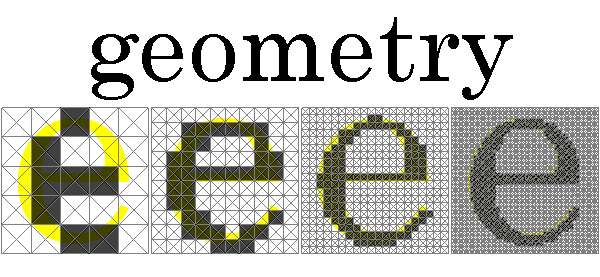
\includegraphics[width=\textwidth]{fig/geometry.pdf}
    % \begin{overpic}[width=0.62\textwidth, abs, grid, unit=0.5in, tics=1]{fig/geometry.pdf}
    % \begin{overpic}[width=0.62\textwidth, abs, unit=0.5in, tics=1]{fig/geometry.pdf}
    % \begin{overpic}[width=0.8\textwidth, abs, grid, unit=0.5in, tics=1]{fig/geometry.pdf}
    \begin{overpic}[width=0.8\textwidth, abs, unit=0.5in, tics=1]{fig/geometry.pdf}
      \put(1.15, 0){10 ppi}
      \put(3.65, 0){20 ppi}
      \put(6.15, 0){40 ppi}
      \put(8.65, 0){80 ppi}
    \end{overpic}
  \end{center}
    \caption{Illustration of vector graphics versus rasterized graphics, and the
    concept of pixel resolution.
    Reference: fig/geometry.pdf}
  \label{fig:geometry_pixels} % label must come after caption 
\end{figure}



\chapter{Non-local Methods}
In the following sections, we introduce non-local methods
to create curves from data points.  Thereafter, we
introduce local methods.
Non-local methods mean that any change in a data point (or a control point) 
affects 
the {\em entire} curve.  This is generally undesirable.  
However, non-local methods are simpler than local methods, so they 
are introduced first.  Table~\ref{tab:concept_map} presents an overview
of the four methods to be covered, categorized by interpolation and 
locality.

\begin{table}[htb]
\caption{Categorization of methods by interpolation and locality.}
% \centering
\begin{center}
\begin{tabular}{cc||c|c}
& & \multicolumn{2}{c}{\bf Locality} \\
& & non-local methods & local methods \\
& & ``curves'' & ``splines'' \\
\hline \hline
\multirow{2}{*}{\bf Interpolation} & data points & polynomial & spline \\ \cline{2-4}
& control points & B\'ezier, Bernstein & B-spline, NURB \\
\end{tabular}
\end{center}
\label{tab:concept_map}
\end{table}
In general, we will refer to non-local methods as {\bf curves} of 
degree $p$, denoted
$f_p(x) \in \real$ for non-parameterized curves (univariate polynomials, as
in Table~\ref{tab:polynomials}) and 
$\vC_p(t; \vx) \in \realthree$ for parameterized curves (B\'ezier curves written
in the Bernstein basis, as in (\ref{eq:general_bezier_curve})).  
In contrast, we will refer to local methods as {\bf splines} of 
degree $p$, denoted $S_p(t; x) \in \real$ and 
$\vS_p(t; \vx) \in \realthree$ (used throughout Chapter~\ref{chapter:local_methods}).

\section{Polynomials}
We briefly discuss polynomials for three main reasons:  
(1)~To be explicit
regarding the terminology of {\bf power} versus {\bf order} and be clear
on the conventions and notations used in this document, 
(2)~to lay the framework
for more sophisticated interpolations that will rely on polynomials in some 
form, and 
(3)~to
the  note shortcomings of polynomials and thus motivate alternative 
approaches.

First, with regard to {\em power} versus {\em order}, \cite{Cottrell-2009}
noted the following:

\begin{Hquote}
Page 18, Note 3: ``There is a terminology conflict between the geometry and analysis communities. 
Geometers will say a cubic polynomial has degree 3 and order 4.  In geometry,
order equals degree plus one.  Analysts will say a cubic polynomial is order
three, and use the term order and degree synonymously.  This is the convention
we [Cottrell, Hughes, Bazilevs] adhere to.'' 
\end{Hquote}

Unlike \cite{Cottrell-2009}, we adopt the geometry community 
convention in this document, thus 
we distinguish between {\em order} and {\em power}.  
We have elected this approach primarily for consistency of this 
document with historical writings of the geometry community.

Next, there is some basic notation used with polynomials that we need 
to make clear and concrete.  
Let $f_p(x)$ be the function of degree $p$ 
(equivalently, order $p+1$) that is a sum of variable
$x$ raised to some increasing non-negative integer power, starting 
from zero, and multiplied
by a constant coefficient $a$, such that
\be
f_p(x) \defe
a_0 x^0 + a_1 x^1 + a_2 x^2 + a_3 x^3 + \cdots + a_p x^p = 
\sum_{i=0}^p a_i x^i.
\ee
The function $f_p(x)$ is a {\bf polynomial} of {\bf degree} $p$, the highest
non-zero {\bf power}\footnote{We suggest the mnemonic of ``$p$'' as the 
index used for the ``\underline{p}ower'' in a ``\underline{p}olynomial.''} used in the summation.  
Table~\ref{tab:polynomials} lists
the first five polynomials by order, degree, name, and function.  
Hereinafter, $p$ will be considered the index of the 
power of a polynomial.  The $p$-index, a subset of non-negative integers, 
will start from zero and consecutively increase by one.

\begin{table}[htb]
\caption{First five orders of a polynomial function.}
% \centering
\begin{center}
\begin{tabular}{c|c|l|l}
{\bf order} & {\bf degree} & {\bf name} & {\bf function} \\
\hline \hline
$\mathcal{O}(1)$ & $p=0$ & constant & $f_0(x) = a_0$ \\
$\mathcal{O}(2)$ &  $p=1$ & linear & $f_1(x) = a_0 + a_1 x$ \\
$\mathcal{O}(3)$ & $p=2$ & quadratic & $f_2(x) = a_0 + a_1 x + a_2 x^2$ \\
$\mathcal{O}(4)$ & $p=3$ & cubic & $f_3(x) = a_0 + a_1 x + a_2 x^2 + a_3 x^3$ \\
$\mathcal{O}(5)$ & $p=4$ & quartic & $f_4(x) = a_0 + a_1 x + a_2 x^2 + a_3 x^3 + a_4 x^4$ \\
\end{tabular}
\end{center}
\label{tab:polynomials}
\end{table}

One note regarding conventions of indices.  We use the first
item of a series {\tt s} to be {\tt s[0]}, the second item to be 
{\tt s[1]}, and so forth.  We prefer the zero-based indices because 
it is consistent not only with our work in Python, which is zero-based, 
but also with concepts from initial boundary value problems (IBVPs), 
which denote initial conditions, the first values, as occurring at $t_0$.

Finally, we state as {\em prima facie} a well-known shortcoming of polynomials
is their propensity to overfit the data.  This characteristic arises because
a polynomial of degree $p$ has $p-1$ changes of direction, from $-f_p(x)$ to
$f_p(x)$, or vice versa.  No further discussion on overfitting is given here, 
though explications of this topic are widely available.  


\section{B\'ezier Curves}
\label{sec:bezier_curves}
Several of the ideas in this section are due to the excellent references
of \cite{Bartels-1995}, \cite{Piegl-2012}, \cite{Rogers-2000}, 
and \cite{Shiach-2015}.
A B\'ezier curve is a parametric curve defined by control points.
A control point $\vP_i$ will have two coordinates $(x_i, y_i)$ in 2D and
three coordinates $(x_i, y_i, z_i)$ in 3D.
The parameter is typically denoted $t$.  The bounds for $t$ are 
$0 \leq t \leq 1$ unless otherwise indicated.

Here, $t$ does not denote time, as is customary in solid mechanics.  
Rather, $t$ can be thought of as a ``pseudo-time,'' wherein the 
parameterization flows from beginning to end of the $t$ bounds.
Also, the bounds of $t$ will later be shown to be arbitrary.  For now, 
however, it is much more convenient to state the bounds as between zero
and one.

A B\'ezier curve of degree $p$ requires $p+1$
control points. For example, a B\'ezier 
curve that is a line (degree $p=1$) requires two control points.
Affine transformations may be used to modify the control points, \eg to 
scale, reflect, rotate, or translate (offset) the control points.

\subsection{B\'ezier Line}
Let $\vP(t; \vx) \in \realthree$ be {\bf parametric} equation for a line between 
two points $\vP_0 = (x_0, y_0, z_0)$ and $\vP_1 = (x_1, y_1, z_1)$, with
$\vx = (x, y, z)$.
Then, let $t$ be the parameter bounded by $0 \leq t \leq 1$.  Then 
the B\'ezier line between $\vx_0$ and $\vx_1$ is simply the parameterized 
linear interpolation $\vP_0$ and $\vP_1$, 
\be
\vP(t; \vP_0, \vP_1) \defe (1 - t) \vP_0 + t \vP_1, 
\ee
or in explicit coordinate form,
\be
\left\{\begin{tabular}{c} $x(t)$ \\ $y(t)$ \\ $z(t)$ \end{tabular} \right\}
= 
(1 - t)
\left\{\begin{tabular}{c} $x_0$ \\ $y_0$ \\ $z_0$ \end{tabular} \right\}
+ 
t \left\{\begin{tabular}{c} $x_1$ \\ $y_1$ \\ $z_1$ \end{tabular} \right\}.
\ee

\subsection{B\'ezier Quadratic}
Let $\vQ(t; \vx)$ be the parametric equation for a quadratic between two points
$\vQ_0$ and $\vQ_1$.  Let the position of these two points themselves be 
parameterized by three points $\vP_0$, $\vP_1$, and $\vP_2$, such that
\begin{align}
\vQ_0(t; \vP_0, \vP_1) & = (1 - t) \vP_0 + t \vP_1,
\label{eq:bezier_quad_one}
\\
\vQ_1(t; \vP_1, \vP_2) & = (1 - t) \vP_1 + t \vP_2.
\label{eq:bezier_quad_two}
\end{align}
Thus, the position of $\vQ_0$ is on the line between points $\vP_0$ and 
$\vP_1$.  The position of $\vQ_1$ is on the line between points $\vP_1$ and 
$\vP_2$.
At $t=0$, $\vQ_0$ resides at $\vP_0$, $\vQ_1$ resides at $\vP_1$.  
At $t=1$, $\vQ_0$ resides at $\vP_1$, $\vQ_1$ resides at $\vP_2$.
Finally, let position along the quadratic B\'ezier curve $\vQ(t; \vx)$ 
be defined as 
\be
\vQ(t; \vQ_0, \vQ_1) \defe (1 - t) \vQ_0 + t \vQ_1.
\ee
This curve can be recast in terms of the three points $\vP_0$, $\vP_1$, 
and $\vP_2$ by substituting
(\ref{eq:bezier_quad_one}) and
(\ref{eq:bezier_quad_two}),
\be
\vQ(t; \vP_0, \vP_1, \vP_2) = (1-t)^2 \vP_0 + 2t (1-t) \vP_1 + t^2 \vP_2.
\label{eq:bezier_quadratic}
\ee
Figure~\ref{fig:de_casteljau}(a) illustrates 
an example quadratic B\'ezier curve, with the three control 
points $\vP_0$, $\vP_1$, and $\vP_2$ indicated.\footnote{We do
not call $\vQ_0$ and $\vQ_1$ control points, since they are dependent
on $\vP_0$, $\vP_1$, and $\vP_1$ through parameter $t$ in 
(\ref{eq:bezier_quad_one}) 
and (\ref{eq:bezier_quad_two}).}$^,$\footnote{Figure~\ref{fig:de_casteljau}(b)
shows the same curve as in Figure~\ref{fig:de_casteljau}(a), just with 
a recursive notation, discussed in Section~\ref{sec:de_casteljau}.}
We will designate the number of control points to be $(n+1)$.  
Thus, the number of control points in the 
current example (Figure~\ref{fig:de_casteljau})
is $(n+1) = 3 \implies n=2$.  Each control
point can be identified in sequence as $\vP_i$, with $i = 0, 1, \ldots n$.
The maximum 
degree B\'ezier that can be constructed is two 
(degree $p$ requires $p+1$ control points).  Thus we see 
for a series of $(n+1)$ control points, we can construct a 
B\'ezier curve of degree $p=n$.

\begin{figure}[htb]
  \begin{center}
    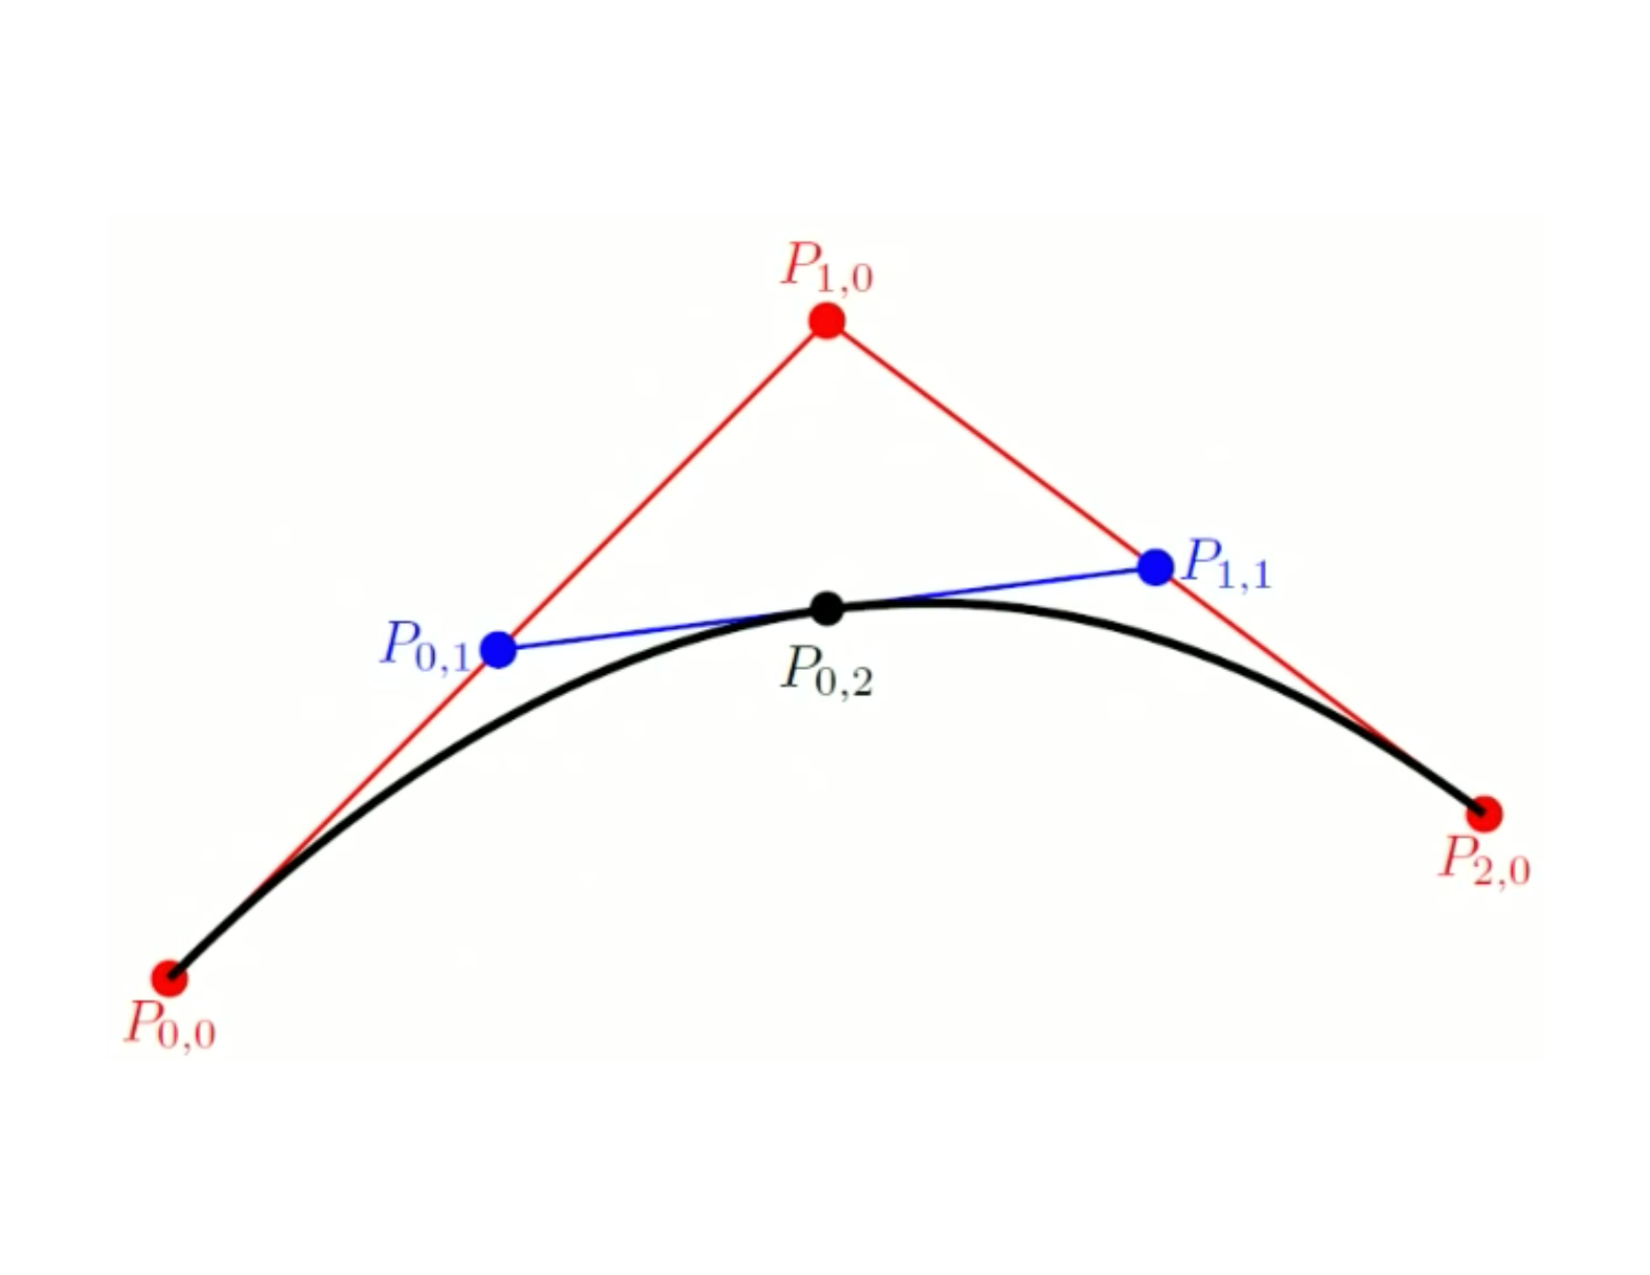
\includegraphics[width=\textwidth]{fig/de_casteljau.pdf}
  \end{center}
    \caption{A B\'ezier quadratic curve illustrated at $t=0.5$
    with (a) original notation 
    and (b) the de Casteljau's algorithm notation.  
    Reference: fig/de\_casteljau.py.}
  \label{fig:de_casteljau} % label must come after caption 
\end{figure}

\begin{Hexpo}
{Figure~\ref{fig:de_casteljau_sequence} illustrates the same quadratic
B\'ezier curve shown in Figure~\ref{fig:de_casteljau}, generated at  
six discrete points in the interval $t \in [0, 1]$.
\begin{figure}[htb]
  \begin{center}
    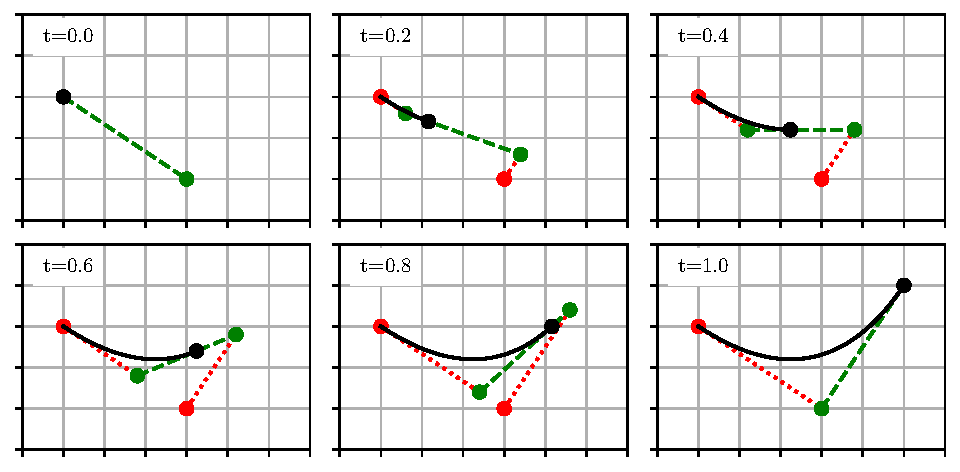
\includegraphics[width=\textwidth]{fig/de_casteljau_sequence.pdf}
  \end{center}
    \caption{The B\'ezier quadratic curve discussed in 
    Figure~\ref{fig:de_casteljau}, 
    illustrated in sequence with $t$ starting at 0 and ending at 1.
    Reference: fig/de\_casteljau.py.}
  \label{fig:de_casteljau_sequence} % label must come after caption 
\end{figure}
}
\end{Hexpo}

With these Figures~\ref{fig:de_casteljau}--\ref{fig:de_casteljau_sequence} 
in mind, a few additional observations\footnote{These items
are stated as true but not proven here. Consult
the references in the Bibliography section for proofs.} can be made:
\begin{itemize}
 \item The control points sequence $\vP_0$, $\vP_1$, $\vP_2$ is a coarse 
 and discrete {\em approximation} the continuous quadratic B\'ezier curve
 $\vQ(t)$.
 \item The end points, $\vP_0$ and $\vP_2$, are interpolated, but 
 the interior point $\vP_1$ is not
 interpolated.\footnote{This will generalize to all interior points for
 higher-degree B\'ezier curves.}
 \item The tangent of the curve $\vQ(t)$ at $t=0$ is parallel to the line
 $\vP_1 - \vP_0$.
 The tangent of the curve $\vQ(t)$ at $t=1$ is parallel to the line
 $\vP_2 - \vP_0$.
 \item The entire curve $\vQ(t)$ is contained in the triangle formed with vertices
 $\vP_0$, $\vP_1$, $\vP_2$.
\end{itemize}




\newpage
\subsection{de Casteljau's Algorithm}
\label{sec:de_casteljau}
The foregoing development can be generalized, and is known as 
{\bf de Casteljau's algorithm}.  Let $\vP_{i,j}$ be control points
where 
\begin{itemize}
\item $i$ denotes the {\bf control point index}, $i=0, 1, \ldots n$, (total 
of $n+1$ control points), and
\item $j$ denote the {\bf degree} of the curve, $j=0, 1, \ldots p$.
\end{itemize}
Thus $\vP_{i,0}$ denote the base level control points. 
In the preceding section, 
\begin{align}
\vP_0 & \mapsto \vP_{0,0}, \;\;\;\mbox{$j=0$, thus $\vP_{i,0}$ is a point,}\\
\vP_1 & \mapsto \vP_{1,0}, \\
\vP_2 & \mapsto \vP_{2,0}, \\
 & \nonumber \\
\vQ_0 & \mapsto \vP_{0,1}, \;\;\;\mbox{$j=1$, thus $\vP_{i,1}$ is a line,}\\
\vQ_1 & \mapsto \vP_{1,1}, \;\;\;\mbox{and} \\
 & \nonumber \\
\vQ(t) & \mapsto \vP_{0,2}, \;\;\;\mbox{$j=2$, thus $\vP_{i,2}$ is a quadratic.}
\end{align}
Then, {\bf de Casteljau's algorithm} states
\be
\vP_{i,j} = (1-t) \vP_{i,j-1} + t \vP_{i+1, j-1}.
\ee
Equation~(\ref{eq:bezier_quadratic}) would then be rewritten as
\begin{align}
\vP_{0,2}(t)
& = (1-t) \vP_{0,1} + t \vP_{1,1}, \\
& = (1-t) \left[ (1-t) \vP_{0,0} + t \vP_{1,0} \right] + 
    t     \left[ (1-t) \vP_{1,0} + t \vP_{2,0} \right], \\
& = (1-t)^2 \vP_{0,0} + 
2t (1-t) \vP_{1,0} + t^2 \vP_{2,0},
\label{eq:quadratic_bezier}
\end{align}
where only the $t$ parameter is used to describe $\vP_{0,2}(\cdot)$ for the 
sake of brevity.  Figure~\ref{fig:de_casteljau} illustrates for the B\'ezier
quadratic development, (a) the original notation and (b) the de 
Casteljau's algorithm notation.

For efficiency during computational implementation, 
it is common to rewrite the quadratic B\'ezier $\vP_{0,2}$ 
in matrix form for {\bf any sequence} of {\bf three control 
points}\footnote{This is 
somewhat of a 
return map, undoing the notation adopted to
explain de~Casteljau's algorithm 
with $i = 0$.}
$\vP_i$, $\vP_{i+1}$, and $\vP_{i+2}$.
With
\begin{align}
\vP_{0,0} & \mapsto \vP_i, \\
\vP_{1,0} & \mapsto \vP_{i+1}, \\
\vP_{2,0} & \mapsto \vP_{i+2}, \mbox{ and } \\
\vP_{0,2} & \mapsto \vC_2, \mbox{ to denote a curve } \vC_p \mbox { of degree } p=2,
\end{align}
the quadratic B\'ezier $\vC_2$ is written in matrix form as
\begin{align}
\vC_2(t) \;\;\;\;\; & = \; \left[\;\; \vP_i \;\;\; \vP_{i+1} \;\;\; 
\vP_{i+2} \;\; \right] 
\; \cdot \; \vf(t^2, t, 1),
\\
\left\{\begin{tabular}{c} $x(t)$ \\ $y(t)$ \\ $z(t)$ \end{tabular} \right\}
% \vC_2(t) 
& = 
% \left\{\begin{tabular}{c} $x(t)$ \\ $y(t)$ \\ $z(t)$ \end{tabular} \right\}
% = 
\underset{\underset{\mbox{\footnotesize curve dependent}}{\mbox{\footnotesize control points}}}{% underset open
%\underset{\mbox{\footnotesize control points}}{% underset open
\underbrace{% underbrace open
\left[\begin{tabular}{ccc} 
$x_i$ 
& 
$x_{i+1}$ 
& 
$x_{i+2}$ 
\\ 
$y_i$ 
& 
$y_{i+1}$ 
& 
$y_{i+2}$ 
\\ 
$z_i$ 
& 
$z_{i+1}$ 
& 
$z_{i+2}$ 
\end{tabular} \right]
}% underbrace close
}% underset close
%
\;\;\;
\underset{\mbox{\footnotesize curve independent}}{% underset open
\underbrace{% underbrace open
\left[\begin{tabular}{crr} 
1 
& 
-2
& 
1
\\ 
% 
& 
2
& 
0
\\ 
sym.
& 
%
& 
0
\end{tabular} \right]
%
\left\{\begin{tabular}{c} $t^2$ \\ $t$ \\ $1$ \end{tabular} \right\}
}% underbrace close
}% underset close
.
\end{align}


\subsection{B\'ezier Cubic}
The cubic B\'ezier curve $\vP_{0,3}(t)$, given four control points
$\vP_{0,0}$,
$\vP_{1,0}$,
$\vP_{2,0}$, and
$\vP_{3,0}$,
is given by
\be
\vP_{0,3}(t) = 
(1-t)^3 \vP_{0,0} + 
3t(1-t)^2 \vP_{1,0} + 
3t^2 (1-t) \vP_{2,0} + 
t^3 \vP_{3,0}.
\label{eq:bezier_cubic}
\ee
Again for efficiency, 
it is common to rewrite the cubic B\'ezier $\vP_{0,3}$ 
in matrix form for {\bf any sequence} of {\bf four control 
points}
$\vP_i$, $\vP_{i+1}$, $\vP_{i+2}$ and $\vP_{i+3}$.
With
\begin{align}
\vP_{0,0} & \mapsto \vP_i, \\
\vP_{1,0} & \mapsto \vP_{i+1}, \\
\vP_{2,0} & \mapsto \vP_{i+2}, \\
\vP_{3,0} & \mapsto \vP_{i+3}, \mbox{ and } \\
\vP_{0,3} & \mapsto \vC_3, \mbox{ to denote a curve } \vC_p \mbox { of degree } p=3,
\end{align}
the cubic B\'ezier $\vC_3$ is written in matrix form as
\begin{align}
\vC_3(t) \;\;\;\;\; 
&= 
\left[\;\; \vP_i \;\;\; \vP_{i+1} \;\;\; \vP_{i+2} \;\;\; \vP_{i+3}
\;\; \right] \; \cdot \; \vf(t^2, t, 1),
\\
\left\{\begin{tabular}{c} $x(t)$ \\ $y(t)$ \\ $z(t)$ \end{tabular} \right\}
&= 
\underset{\underset{\mbox{\footnotesize curve dependent}}{\mbox{\footnotesize control points}}}{% underset open
\underbrace{% underbrace open
\left[\begin{tabular}{cccc}
$x_i$ 
& 
$x_{i+1}$ 
& 
$x_{i+2}$ 
& 
$x_{i+3}$ 
\\ 
$y_i$ 
& 
$y_{i+1}$ 
& 
$y_{i+2}$ 
& 
$y_{i+3}$ 
\\ 
$z_i$ 
& 
$z_{i+1}$ 
& 
$z_{i+2}$ 
& 
$z_{i+3}$ 
\end{tabular} \right]
}% underbrace close
}% underset close
%
\;\;\;
\underset{\mbox{\footnotesize curve independent}}{% underset open
\underbrace{% underbrace open
\left[\begin{tabular}{crrr}
-1 
& 
3
& 
-3
&
1
\\ 
% 
& 
-6
& 
3
&
0
\\ 
%
& 
% 
&
0
& 
0
\\
sym.
& 
% 
& 
% 
& 
0
\end{tabular} \right]
%
\left\{\begin{tabular}{c} $t^3$ \\ $t^2$ \\ $t$ \\ $1$ \end{tabular} \right\}
}% underbrace close
}% underset close
.
\end{align}


\subsection{Bernstein Polynomials}
The general form of a degree $p$ B\'ezier curve $\vC_p(t)$ defined by 
$p + 1$ control points $\vP_i$, $i=0, 1, \ldots,p$, is given by
\be
\vC_p(t) \defe \sum_{i=0}^p b_{i,p}(t) \vP_i,
\label{eq:general_bezier_curve}
\ee
where
$b_{i,p}(t)$ is a {\bf Bernstein polynomial}, defined as
\be
b_{i,p}(t) = 
\left(
\begin{tabular}{c}
$p$ \\ 
$i$
\end{tabular}
\right) 
t^i (1-t)^{p-i}, \;\;\mbox{ and where } \;\;
\left(
\begin{tabular}{c}
$p$ \\ 
$i$
\end{tabular}
\right)
= \dst\frac{p!}{i!\; (p-i)!}
\ee
is the {\bf binomial coefficient}.
The binomial coefficients are readily 
attained from {\bf Pascal's triangle}, written up to $p=4$ in
Table~\ref{tab:pascal}.

\begin{table}[htb]
\caption{First five degrees of binomial coefficients from Pascal's triangle.}
% \centering
\begin{center}
\begin{tabular}{c|ccccccccc}
{\bf degree} & \multicolumn{9}{c}{\bf binomial coefficient} \\
\hline \hline
$p=0$ & & & & & 1 & & & & \\
$p=1$ & & & & 1 &  & 1 & & & \\
$p=2$ & & & 1 & & 2 & & 1 & & \\
$p=3$ & & 1 & & 3 & & 3 & & 1 & \\
$p=4$ & 1 & & 4 & & 6 & & 4 & & 1
\end{tabular}
\end{center}
\label{tab:pascal}
\end{table}

Using (\ref{eq:general_bezier_curve}),
the quadratic ($p=2$), cubic ($p=3$), and quartic ($p=4$) B\'ezier curves
can be written, respectively, in explicit form as 
\begin{align}
\vC_2(t) 
&=
b_{0,2} \vP_0 + b_{1,2} \vP_1 + b_{2,2} \vP_2, \\
\vC_3(t) 
&=
b_{0,3} \vP_0 + b_{1,3} \vP_1 + b_{2,3} \vP_2 + b_{3,3} \vP_3, \\
\vC_4(t) 
&=
b_{0,4} \vP_0 + b_{1,4} \vP_1 + b_{2,4} \vP_2 + b_{3,4} \vP_3 + b_{4,4} \vP_4.
\end{align}
Observations\footnote{See Bibliography for references containing 
proofs.} include (see Figure~\ref{fig:bernstein} for a visual illustration of these 
properties):
\begin{itemize}
\item The Bernstein polynomials always sum to one, 
\be
\sum_{i=0}^p b_{i,p}(t) = 1.0.
\ee
This concept is called {\bf partition of unity}.  
\item The first basis is unity $b_{0,p}(0) = 1$ at the start of the interval $t=0$,
when all other bases are zero.  Similarly, the last basis is unity  
$b_{p,p}(1) = 1$ and the end of the interval $t=1$, when all other bases go to zero.
\item The polynomials are {\bf non-negative},
\be
b_{i,p}(t) \geq 0 \mbox{ for all} \left\{i,p\right\} \mbox{ with } t \in [0, 1].
\ee
\item Each polynomial $b_{i,p}(t)$ has a single maximum in the parameter space 
$t \in [0,1]$ at $t=i/p$.  
\item All polynomials are symmetric in $t$ about $t=1/2$.
\end{itemize}


\clearpage
\begin{Hexpo}
{The Bernstein polynomials for a cubic ($p=3$) B\'ezier curve are
\begin{align}
b_{0,3}(t) & = \left(\begin{tabular}{c} 3 \\ 0 \end{tabular} \right) 
t^0 (1-t)^{3-0} = (1 - t)^3,
\\
%
b_{1,3}(t) & = \left(\begin{tabular}{c} 3 \\ 1 \end{tabular} \right) 
t^1 (1-t)^{3-1} = 3t (1 - t)^2,
\\
%
b_{2,3}(t) & = \left(\begin{tabular}{c} 3 \\ 2 \end{tabular} \right) 
t^2 (1-t)^{3-2} = 3 t^2 (1 - t),
\\
%
b_{3,3}(t) & = \left(\begin{tabular}{c} 3 \\ 3 \end{tabular} \right) 
t^3 (1-t)^{3-3} = t^3,
%
\end{align}
which match the coefficients in (\ref{eq:bezier_cubic}).  
These polynomials are shown in Figure~\ref{fig:bernstein}(c).
} % end Hexpo
\end{Hexpo}

\begin{Hexpo}
{The Bernstein polynomials for a quartic ($p=4$) B\'ezier curve are
\begin{align}
b_{0,4}(t) & = \left(\begin{tabular}{c} 4 \\ 0 \end{tabular} \right) 
t^0 (1-t)^{4-0} = (1 - t)^4,
\\
%
b_{1,4}(t) & = \left(\begin{tabular}{c} 4 \\ 1 \end{tabular} \right) 
t^1 (1-t)^{4-1} = 4 t (1 - t)^3,
\\
%
b_{2,4}(t) & = \left(\begin{tabular}{c} 4 \\ 2 \end{tabular} \right) 
t^2 (1-t)^{4-2} = 6 t^2 (1 - t)^2,
\\
%
b_{3,4}(t) & = \left(\begin{tabular}{c} 4 \\ 3 \end{tabular} \right) 
t^3 (1-t)^{4-3} = 4 t^3 (1 - t),
\\
%
b_{4,4}(t) & = \left(\begin{tabular}{c} 4 \\ 4 \end{tabular} \right) 
t^4 (1-t)^{4-4} = t^4.
\end{align}
These polynomials are shown in Figure~\ref{fig:bernstein}(d).
} % end Hexpo
\end{Hexpo}

\begin{figure}[htb]
  \begin{center}
    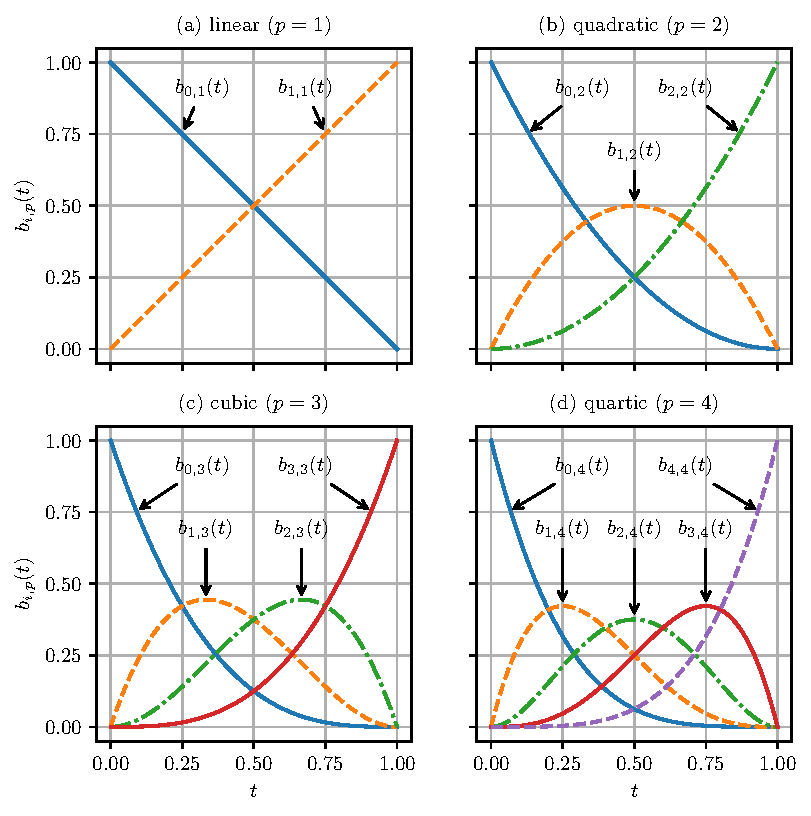
\includegraphics[width=\textwidth]{fig/bernstein.pdf}
  \end{center}
    \caption{Bernstein polynomials for B\'ezier (a) linear, 
    (b) quadratic, 
    (c) cubic, and
    (d) quartic curves.
    Reference: fig/bernstein.py.}
  \label{fig:bernstein} % label must come after caption 
\end{figure}


\clearpage
\section{B\'ezier Surfaces}
The B\'ezier curve was parameterized by $t$.  For the
B\'ezier surface, we have two parameters, $u$ and $v$.
More to come.



\chapter{Local Methods}
\label{chapter:local_methods}
Local methods mean that any change in a control point does not necessarily
affects 
the {\em entire} parameterization.  This is generally very desirable, as
changes can be focused on a specific region, without
disrupting the balance of the parameterization.
However, local methods are more complicated than non-local methods, 
and require definition over intervals, as well be seen below.

\section{General Splines}
Let a collection of $n+1$ points $(x_i, y_i)$ for $ i=0, 1, \ldots, n$ 
approximate the function $y=f(x)$ over the domain $[x_0, x_n]$.  In total, 
there are $n+1$ points and $n$ intervals.  
Let $S(x)$ be the piecewise continuous spine that
threads through each of the points $(x_i, y_i)$.  
For $x \in [x_i, x_{i+1}]$ and  $i=0, 1, \ldots, n-1$, 
the spline takes on $n$ 
interval definitions as follows: 
\be
S_i(x) 
\defe a_i + b_i (x - x_i) + c_i (x - x_i)^2 
+ d_i (x - x_i)^3 + 
\cdots + z_i (x - x_i)^p. 
\ee
where constant coefficients\footnote{Here the $z_i$
is arbitrary, meant to denote the last coefficient, but not necessarily the 
twenty-sixth coefficient.}
multiply successive powers\footnote{The powers are non-negative integers.} 
of $(x-x_i$), summed
to an arbitrary polynomial power $p$.  This is referred to as the {\bf
interval spline definition} to polynomial degree $p$.
Below we consider linear splines ($p=1$), quadratic splines ($p=2$), and
cubic splines ($p=3$).

\section{Linear Splines}
For linear splines, the interval spline definition is
\be
S_i(x) 
\defe
a_i + b_i (x - x_i)
\;\;\;
\mbox{for}
\; x \in [x_i, x_{i+1}] \;\mbox{and}\; i=0, 1, \ldots, n-1.
\ee
For any collection of points $(x_i, y_i)$, all coefficients $a_i$ and
$b_i$ for $i=0, 1, \ldots, n-1$ can be found using the {\bf zeroth derivative
continuity constraint}, which creates a spline that connects to each point
at the beginning and end of each interval, thus
\be
S_i(x_i) = y_i 
\;\;\;
\mbox{and}
\;\;\; 
S_i(x_{i+1}) = y_{i+1}
\;\;\;\mbox{for}\;i=0, 1, \ldots, n-1.
\ee
Here we see there are two constraints per interval $i$ and two unknowns, 
$a_i$ and $b_i$, per interval $i$.  The unknowns can be found directly by
evaluating the interval spline definition with each of the two constraint
equations.  In turn, these are, for 
$i=0, 1, \ldots, n-1$,
\begin{align}
S_i(x_i) 
&
= a_i + b_i(x_i - x_i) 
\overset{\mbox{\footnotesize set}}{=} y_i 
\implies 
a_i = y_i, \;\mbox{and}
\\
S_i(x_{i+1}) 
& 
= a_i + b_i (x_{i+1} - x_i) 
\overset{\mbox{\footnotesize set}}{=} y_{i+1}
\implies
b_i = \frac{y_{i+1} - y_i}{x_{i+1} - x_i}.
\end{align}
No additional continuity constraints can be created since the linear
spline has only $C^0$ continuity, meaning no derivatives of the 
function $S_i(x)$ are continuous.

\begin{Hexpo}
{Let $y = f(x) = \sin(\pi x)$ for $x \in [0, 1]$ be approximated by a linear
spline and a collection of three points equally spaced on the domain.  
Note $n+1 = 3$, thus $n=2$, indicating three points and two intervals.
Table~\ref{tab:linear_spline_example} summarizes the spline data.
Figure~\ref{fig:linear_spline_example}(a) shows the $\sin$ function and the
linear spline interpolations.
\begin{table}[h]
\caption{Linear spline approximation of $y = f(x) = \sin(\pi x)$ 
using three points and two intervals.}
% \centering
\begin{center}
\begin{tabular}{c|c|ccc|ccc}
$i$ & $x_i$ & $y_i$ & $\implies$  & $a_i$ & $b_i$ & $\implies$ & $S_i(x)$
\\
\hline \hline
0 & 0/2 & 0 &  & 0 & 2 &   & $2 x$
\\
1 & 1/2 & 1 &  & 1 & -2 &   & $1 - 2(x - 1/2)$
\\
2 & 2/2 & 0 &  & --- & --- &   & ---
\end{tabular}
\end{center}
\label{tab:linear_spline_example}
\end{table}
} % end Hexpo
\end{Hexpo}

\newpage
\begin{Hexpo}
{Repeat the previous example, but now with a
collection of five points equally spaced on the domain.  
Thus $n+1 = 5$, thus $n=4$, indicating five points and four intervals.
Table~\ref{tab:linear_spline_example_two} summarizes the spline data.
Figure~\ref{fig:linear_spline_example}(b) shows the $\sin$ function and the
linear spline interpolations.
\begin{table}[h]
\caption{Linear spline approximation of $y = f(x) = \sin(\pi x)$ 
using five points and four intervals.}
% \centering
\begin{center}
\begin{tabular}{c|c|ccc|ccc}
$i$ & $x_i$ & $y_i$ & $\implies$  & $a_i$ & $b_i$ & $\implies$ & $S_i(x)$
\\
\hline \hline
0 & 0/4 & 0 &  & 0 & $2\sqrt{2}$ &   & $2\sqrt{2} x$
\\
1 & 1/4 & $\sqrt{2}/2$ &  & $\sqrt{2}/2$ & $4 - 2\sqrt{2}$ &   
& $\sqrt{2}/2 + (4-2\sqrt{2})(x - 1/4)$
\\
2 & 2/4 & 1 &  & 1 & $2\sqrt{2} - 4$ &   & $1 + (2\sqrt{2}-4)(x - 2/4)$
\\
3 & 3/4 & $\sqrt{2}/2$ &  & $\sqrt{2}/2$ & $-2\sqrt{2}$ &   & $\sqrt{2}/2 - 
2\sqrt{2}(x - 3/4)$
\\
4 & 4/4 & 0 &  & --- & --- &   & ---
\end{tabular}
\end{center}
\label{tab:linear_spline_example_two}
\end{table}
} % end Hexpo
\end{Hexpo}

% \clearpage
\begin{figure}[htb]
  \begin{center}
    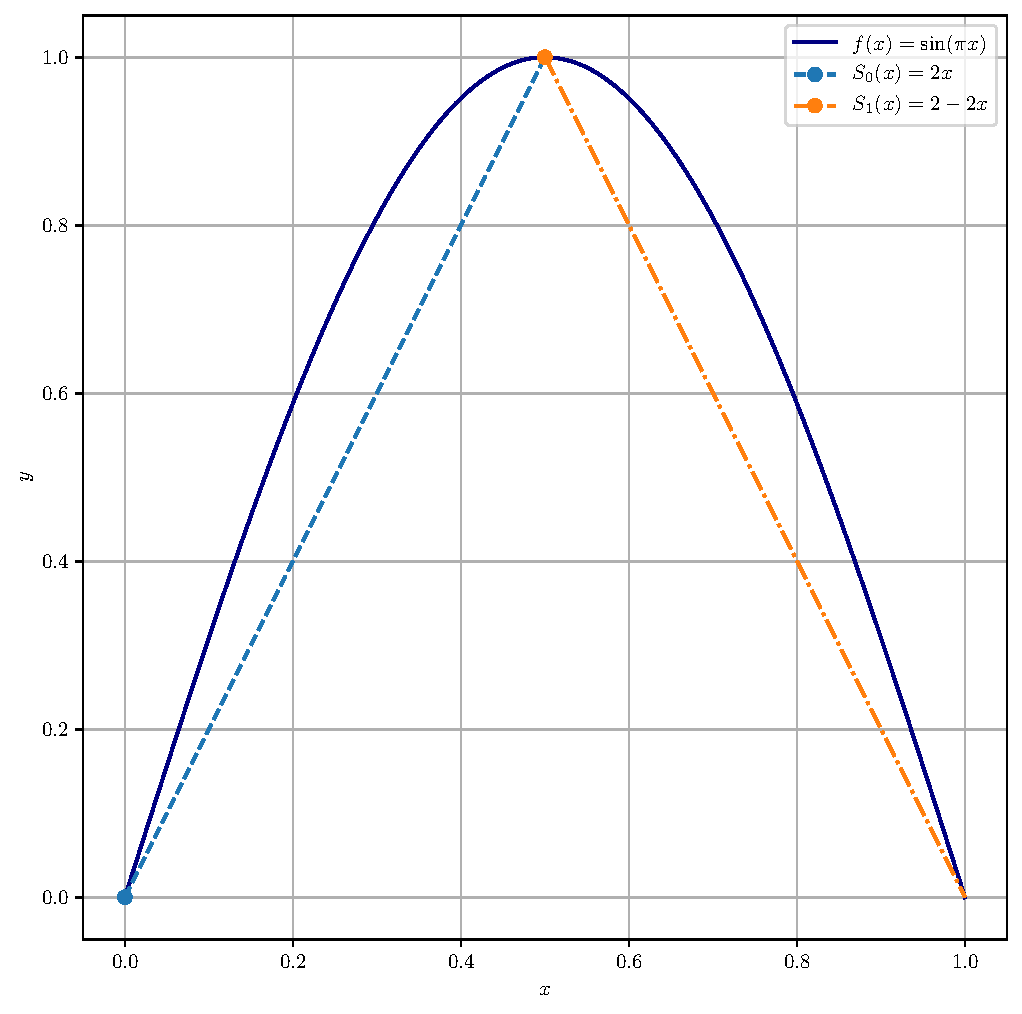
\includegraphics[width=\textwidth]{fig/linear_spline.pdf}
  \end{center}
    \caption{Linear spline example (a) with three points and (b) with five 
    points, see Table~\ref{tab:linear_spline_example_two} for individual 
    definitions of $S_i(x)$.
    Reference: fig/linear\_spline.py.}
  \label{fig:linear_spline_example} % label must come after caption 
\end{figure}


\clearpage
\section{Quadratic Splines}

For quadratic splines, the interval spline definition is 
\be
S_i(x) \defe a_i + b_i (x - x_i) + c_i (x - x_i)^2
\;\;\;
\mbox{for}
\; x \in [x_i, x_{i+1}] \;\mbox{and}\; i=0, 1, \ldots, n-1.
\ee


\section{Cubic Splines}
Cubic splines are useful because of their inherent smoothness.  
The cubic spline, its first derivative, and its second derivative are all
continuous.  Starting with the cubic spine's third derivative, discontinuity
arises.

Let a collection of $n+1$ points $(x_i, y_i)$ for $ i=0, 1, \ldots, n$ 
approximate the function $y=f(x)$ over the domain $[x_0, x_n]$.  In total, 
there are $n+1$ points and $n$ intervals.  
Let $S(x)$ be the piecewise continuous spine, cubic in this case, that
threads through each of the points $(x_i, y_i)$.  The spline takes on $n$ 
interval definitions as follows: 
\be
S_i(x) \defe a_i + b_i (x - x_i) + c_i (x - x_i)^2 + d_i (x - x_i)^3
\;\;\;
\mbox{for}
\; x \in [x_i, x_{i+1}] \;\mbox{and}\; i=0, 1, \ldots, n-1.
\ee
The $n$ foregoing definitions, with the coefficients $a_i, b_i, c_i, d_i$,
give rise to $4n$ (currently unknown) parameters 
used to define the complete spline $S(x)$.  Note that maintain its cubic nature, 
the spline must have $d_i \neq 0$.

Next we endow the spline with constraints on continuity and differentiability,
which allow the $4n$ unknown parameters to be solved.  First, function
continuity requires that the spline, on a particular interval, thread through
collection of points $(x_i, y_i)$ and the beginning and end of each interval.  
Thus, 
\be
S_i(x_i) = y_i \;\mbox{and}\; S_i(x_{i+1}) = y_{i+1}
\;\;\;\mbox{for}\;i=0, 1, \ldots, n-1.
\ee
This is the {\bf continuity constraint}, 
which gives rise to $2n$ conditions\footnote{Two conditions per interval
times $n$ intervals yields $2n$ conditions.}
and creates a spline that
is piecewise continuous.
Next, consider two {\bf differentiability constraints}, which state that the
first and second derivatives at a point $x_i$ are continuous.  That is, 
the first and second derivatives approaching a point $x_i$ from the interval
to the left side of the point must match the respective first and second 
derivatives
approaching the point $x_i$ from the interval to the right side of the point:
\be
S'_{i-1}(x_i) = S'_{i}(x_i) 
\;\mbox{and}\; 
S''_{i-1}(x_i) = S''_{i}(x_i) 
\;\;\;\mbox{for}\;i=1, 2, \ldots, n-1.
\ee
Because they apply only to the interior points
(and not the endpoints $x_0$ and $x_n$), the differentiability constraints
give rise to $2(n-1)$ constraints.\footnote{Two conditions per interior
point times $n-1$ interior points yields $2(n-1)$ conditions.}

Finally, two more conditions are necessary to completely define the spline
$S(x)$.  The two conditions are obtained by specifying differentiability
conditions on the two spline endpoints $x_0$ and $x_n$.  
Frequently, the first derivative is set to the known value of the function's
derivatives at the endpoints, 
\be
S'_0(x_0) = f'(x_0) 
\;\mbox{and}\; 
S'_{n-1}(x_n) = f'(x_n).
\ee
This is defined as a {\bf clamped spline}.
Alternatively, a {\bf natural spline} defines the second derivatives to be
zero at the endpoints, 
\be
S''_0(x_0) = 0 
\;\mbox{and}\; 
S''_{n-1}(x_n) = 0.
\ee
Finally, a {\bf not-a-knot} spline requires no additional constraints on the 
endpoint derivatives,\footnote{This has no effect on the original continuity
constraint on the endpoints, that $S_0(x_0) = y_0$ and $S_{n-1}(x_n) = y_n$.}
but requires that the {\em third} derivative be continuous at $x_1$ and 
$x_{n-1}$.

\section{B-Splines}
A {\bf B-spline} is a spline composed of two or more B\'ezier curves, joined 
end-to-end, subject to certain restrictions, which will be discussed below.
The ``B'' in B-spline stands for {\bf basis}, as the spline
curves, defined over an interval, utilize
control points that are interpolated with basis functions.
In contrast, 
general splines (\eg the linear, quadratic, and cubic 
splines discussed in the previous sections)
use data points that are interpolated directly, without basis functions.

B-splines are {\bf parametric}, so the functional form for a general
B-spline curve $\vS \in \realthree$, will will be written
explicitly as $\vS(t; \vx)$, similar to the notation introduced with
the B\'ezier curves in Section~\ref{sec:bezier_curves}.  Similar to
the B\'ezier 
compact notation discussed previously, B-spline 
curves are typically written in terms of the parametric variable $t$, without
the explicit notation of the space coordinates 
$\vx$ of the control points, \ie $\vP_i(\vx) = \langle \; x_i, y_i, z_i
\; \rangle$.

Similar to the definition of a general B\'ezier curve $\vC_p(t)$ of degree
$p$ in (\ref{eq:general_bezier_curve}), the general form for a 
B-spline $\vS_p(t)$ of degree $p$, with $n+1$ (not necessarily $p+1$, as
with B\'ezier curves) control points 
$\vP_i$, $i=0, 1, \ldots, n$, is given by
\be
\vS_p(t) \defe \sum_{i=0}^n N_{i,p}(t) \vP_i, 
\ee
where $N_{i,p}$ is the {\bf normalized basis function} and $\vP_i \in \realthree$
are the control points $\vP_0, \vP_1, \ldots, \vP_n$.
The normalized basis functions are defined by the {\bf Cox-de~Boor recursion
formulas}:
\be
\mbox{for } p=0: \;\;\; N_{i,0}(t) \;\; \defe \;\;
\left\{
\begin{tabular}{cl}
1
&
if $t_i \leq t < t_{i+1}$,
\\
0 
& 
otherwise.
\end{tabular}
\right.
\ee
%
\be
\mbox{for } p\geq 1: \;\;\; 
N_{i,p}(t) \;\; \defe \;\;
\dst\frac{\;\;\;\;t - t_i}{t_{i+p} - t_i} \; N_{i,p-1}(t) 
\;\; + \;\;
\dst\frac{t_{i+p+1} - t\;\;\;\;\;}{t_{i+p+1} - t_{i+1}} \; N_{i+1,p-1}(t).
\ee
The structure of the Cox-de~Boor recursion formulas is shown below through
illustrations of linear ($p=1$), quadratic ($p=2$), and cubic ($p=3$)
examples.
% make sure to break with LF prior to Hexpo
\\  % This is the break
%  
\begin{Hexpo}
{% Hexpo open
Linear B-spline ($p=1$): \\
\be
\mbox{for } p=1: \;\;\;
N_{i,1}(t) = 
\dst\frac{\;\;\;\;t - t_i}{t_{i+1} - t_i} \; N_{i,0}(t) 
\;\; + \;\;
\dst\frac{t_{i+2} - t\;\;\;\;\;}{t_{i+2} - t_{i+1}} \; N_{i+1,0}(t)
\ee
The linear forms are shown in the middle subfigure of Figure~\ref{fig:bspline}.
}% Hexpo close
\end{Hexpo}
\\
%
\begin{Hexpo}
{% Hexpo open
Quadratic B-spline ($p=2$): \\
\be
\mbox{for } p=2: \;\;\;
N_{i,2}(t) = 
\dst\frac{\;\;\;\;t - t_i}{t_{i+2} - t_i} \; N_{i,1}(t) 
\;\; + \;\;
\dst\frac{t_{i+3} - t\;\;\;\;\;}{t_{i+3} - t_{i+1}} \; N_{i+1,1}(t)
\ee
The linear forms are shown in the bottom subfigure of Figure~\ref{fig:bspline}.
}% Hexpo close
\end{Hexpo}
\\
%
\begin{Hexpo}
{% Hexpo open
Cubic B-spline ($p=3$): \\
\be
\mbox{for } p=3: \;\;\;
N_{i,3}(t) = 
\dst\frac{\;\;\;\;t - t_i}{t_{i+3} - t_i} \; N_{i,2}(t) 
\;\; + \;\;
\dst\frac{t_{i+4} - t\;\;\;\;\;}{t_{i+4} - t_{i+1}} \; N_{i+1,2}(t)
\ee
}% Hexpo close
\end{Hexpo}

\begin{figure}[h!]
  \begin{center}
    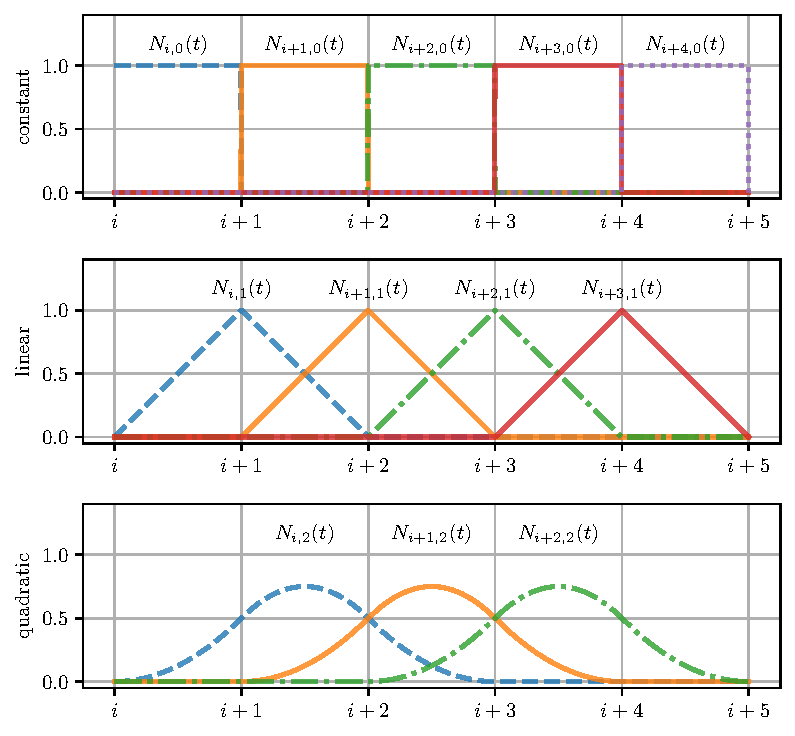
\includegraphics[width=\textwidth]{fig/bspline.pdf}
  \end{center}
    \caption{Normalized basis functions of the Cox-de Boor recursion formula
    for constant, linear, and quadratic forms.
    Reference: fig/bspline.py.}
  \label{fig:bspline} % label must come after caption 
\end{figure}

The discrete values (\eg
$t_i$, $t_{i+1}$, $t_{i+2}$, $t_{i+3}$, $t_{i+4}$, $t_{i+p}$, and $t_{i+p+1}$)
are referred to as {\bf knots}, which
mark the termination points, beginning or end, of an interval for the
parameter $t$.  The collection of all knots is called a {\bf knot vector}, 
designated by $\vT$.
We define the knot vector $\vT$
as a non-decreasing set of non-negative integer coordinates 
in parameter space, 
\be
\vT \defe 
\langle 
\; t_0, t_1, t_2, \ldots, t_m \;
\rangle.
\ee
The values for parameter $t$ are $t \in \real \subset [t_0, t_m]$
In total, there are $(m+1)$ knots in knot vector $\vT$.

\begin{Hexpo}
{% Hexpo open
A uniform knot vector containing 10 knots is written as
\be
\vT = \langle\; 0, 1, 2, 3, 4, 5, 6, 7, 8, 9 \; \rangle, \mbox{ with } 
t \in \real \subset [0, 9].
\ee
}% Hexpo close
\end{Hexpo}




To construct the B-spline $\vS_p(t)$ with normalized basis 
functions $N_{i,p}(t)$,
$(n+1)$ control points 
$\vP_0, \vP_1, \ldots \vP_n$, and degree $p$, exactly $(m+1)$ knots
must be specified.  The number of knots, $(m+1)$, is related to the
number of control points, $(n+1)$, and the degree, $p$, as
\be
m = (n+1) + p.
\ee

Presently, we consider a knot vector in one dimension only. 
Additional dimensions will be discussed later.  Also, for now we will
limit the discussion to a {\bf uniform knot vector}, wherein the distance
between any two consecutive knots is the same,
\be
\Delta t = t_1 - t_0 = t_2 - t_1  = \cdots = t_m - t_{m-1} = 1 = \mbox{constant}.
\ee
Later, we will consider two additional concepts:
{\em repeated} knots and {\em non-uniform} 
knots.\footnote{The variable knot-to-knot distance 
will create a {\bf non-uniform knot vector}, 
which is the ``non-uniform'' of NURBs (non-uniform rational B-splines).}





























\appendix
\appendixpage

\chapter{Code Listing}
\label{chap:code}

\begin{minted}
[
frame=lines,
framesep=2mm,
baselinestretch=1.0,
fontsize=\footnotesize,
linenos
]
{python}
#!/usr/bin/env python3
# bernstein_polynomial.py
import math
import sys
import numpy as np

def bernstein_polynomial(i, p, nti):
    """ 
    Computes the Bernstein polynomial coefficient for 
    control point i with 
    polynomial degreee p
    for a 1D parameter array t in interval [0, 1] broken into 
    nti number of equidistance time intervals.
    """
    if i >= 0 and p >= 1 and nti >= 2 and i <= p:
        t = np.linspace(0, 1, nti+1)
        bp = math.factorial(p) / \
            (math.factorial(i) * math.factorial(p-i)) * t**i * (1-t)**(p-i)
        return bp
    else:
        print(f'Input (i, p, nti) = ({i}, {p}, {nti}) is out of range.')
        print('i is non-negative integer 0, 1, 2, ... p')
        print('p is integer >= 1')
        print('nti is integer >= 2')
        return None
\end{minted}

\begin{minted}
[
frame=lines,
framesep=2mm,
baselinestretch=1.0,
fontsize=\footnotesize,
linenos
]
{python}
#!/usr/bin/env python3
# bernstein_polynomial_test.py
"""
This module is a unit test of the bernstein_polynomial implementation.

To run
$ python bernstein_polynomial_test.py              # terse interaction
$ python -m unittest bernstein_polynomial_test     # default interaction
$ python -m unittest -v bernstein_polynomial_test  # verbose interaction
"""
# standard library imports
import sys
# 
import numpy as np
from unittest import TestCase, main
# 
import bernstein_polynomial as bp

class TestBernstein(TestCase):

    @classmethod
    def setUpClass(cls):
        cls._TOL = 1e-6  # tolerance
        cls._nti = 4  # number of time intervals
        # t, e.g., four intervals, five evaluation points
        cls._t = np.linspace(0, 1, cls._nti+1)
        cls._verbosity = 0

    @classmethod
    def same(cls, a, b):
        same_to_tolerance = False
        l2norm_diff = np.linalg.norm(a - b)

        if cls._verbosity > 0:
            print(f'array a = {a}')
            print(f'array b = {b}')
            print(f'l2norm_diff = {l2norm_diff}')

        if np.abs(l2norm_diff) < cls._TOL:
            same_to_tolerance = True

        return same_to_tolerance

    def test_000_b01(self):
        known = 1 - self._t
        i, p = 0, 1
        calc = bp.bernstein_polynomial(i, p, self._nti)
        self.assertTrue(self.same(known, calc))

    def test_001_b11(self):
        known = self._t
        i, p = 1, 1
        calc = bp.bernstein_polynomial(i, p, self._nti)
        self.assertTrue(self.same(known, calc))

    def test_003_b02(self):
        known = (1 - self._t)**2
        i, p = 0, 2
        calc = bp.bernstein_polynomial(i, p, self._nti)
        self.assertTrue(self.same(known, calc))

    def test_004_b12(self):
        known = 2 * self._t * (1 - self._t)
        i, p = 1, 2
        calc = bp.bernstein_polynomial(i, p, self._nti)
        self.assertTrue(self.same(known, calc))
        
    def test_005_b22(self):
        known = (self._t)**2
        i, p = 2, 2
        calc = bp.bernstein_polynomial(i, p, self._nti)
        self.assertTrue(self.same(known, calc))

    def test_006_b03(self):
        known = (1 - self._t)**3
        i, p = 0, 3
        calc = bp.bernstein_polynomial(i, p, self._nti)
        self.assertTrue(self.same(known, calc))

    def test_007_b13(self):
        known = 3 * self._t * (1 - self._t)**2
        i, p = 1, 3
        calc = bp.bernstein_polynomial(i, p, self._nti)
        self.assertTrue(self.same(known, calc))

    def test_008_b23(self):
        known = 3 * (self._t)**2 * (1 - self._t)
        i, p = 2, 3
        calc = bp.bernstein_polynomial(i, p, self._nti)
        self.assertTrue(self.same(known, calc))
        
    def test_009_b33(self):
        known = (self._t)**3
        i, p = 3, 3
        calc = bp.bernstein_polynomial(i, p, self._nti)
        self.assertTrue(self.same(known, calc))

    def test_010_b04(self):
        known = (1 - self._t)**4
        i, p = 0, 4
        calc = bp.bernstein_polynomial(i, p, self._nti)
        self.assertTrue(self.same(known, calc))

    def test_011_b14(self):
        known = 4 * self._t * (1 - self._t)**3
        i, p = 1, 4
        calc = bp.bernstein_polynomial(i, p, self._nti)
        self.assertTrue(self.same(known, calc))

    def test_012_b24(self):
        known = 6 * (self._t)**2 * (1 - self._t)**2
        i, p = 2, 4
        calc = bp.bernstein_polynomial(i, p, self._nti)
        self.assertTrue(self.same(known, calc))

    def test_013_b34(self):
        known = 4 * (self._t)**3 * (1 - self._t)
        i, p = 3, 4
        calc = bp.bernstein_polynomial(i, p, self._nti)
        self.assertTrue(self.same(known, calc))

    def test_014_b44(self):
        known = (self._t)**4
        i, p = 4, 4
        calc = bp.bernstein_polynomial(i, p, self._nti)
        self.assertTrue(self.same(known, calc))

if __name__ == '__main__':
    main()  # calls unittest.main()
\end{minted}

\begin{minted}
[
frame=lines,
framesep=2mm,
baselinestretch=1.0,
fontsize=\footnotesize,
linenos
]
{python}
#!/usr/bin/env python3
# bernstein_extended.py
import numpy as np
import matplotlib.pyplot as plt
from matplotlib import rc
from matplotlib.ticker import AutoMinorLocator, MultipleLocator

import bernstein_polynomial as bp

LATEX = 1
SERIALIZE = 0

if LATEX:
  rc('font', **{'family': 'serif', 'serif': ['Computer Modern Roman']})
  rc('text', usetex=True)

nts = 101 # number of time steps, include t0 as a step
nti = nts - 1 # number of time intervals
t = np.linspace(0, 1, nts)  # parameterization

# fig = plt.figure(figsize=(6, 6))  # x in inches wide, y inches tall
fig = plt.figure(figsize=(6.5, 6.5))  # x in incmes wide, y inches tall
ax2 = fig.add_subplot(2, 2, 3, aspect=1)
ax0 = fig.add_subplot(2, 2, 1, aspect=1)
ax3 = fig.add_subplot(2, 2, 4, aspect=1, sharey=ax2)
ax1 = fig.add_subplot(2, 2, 2, aspect=1, sharey=ax0, sharex=ax3)

# globals
ap = dict(arrowstyle='->')  # arrow properties
lax, lay = 0.5, 1.1
b0_x = 0.32
b0_y = 0.87
dx = 0.008
annotate_dict = dict(arrowprops=ap, 
    ha='center', 
    va='bottom',
    backgroundcolor='white')
text_dict = dict(ha='center', 
    va='bottom',
    backgroundcolor='white')
linestyle_tuple = ('solid', 'dashed', 'dashdot')

p = 5
for q in np.arange(p+1):
    ls = linestyle_tuple[q % len(linestyle_tuple)]
    ax0.plot(t, bp.bernstein_polynomial(q, p, nti), linestyle=ls)

ax0.annotate(r'$b_{0,5}(t)$', xy=(0.06-dx, 0.75), xytext=(b0_x, b0_y), **annotate_dict)
ax0.text(lax, b0_y, r'$\ldots$', **text_dict)
ax0.annotate(r'$b_{5,5}(t)$', xy=(0.94+dx, 0.75), xytext=(1-b0_x, b0_y), **annotate_dict)

ax0.xaxis.set_major_locator(MultipleLocator(0.25))
ax0.yaxis.set_major_locator(MultipleLocator(0.25))
ax0.set_ylabel(r'$b_{i,p}(t)$')
ax0.text(lax, lay, r'(a) $p=5$', **text_dict)
ax0.grid()
plt.setp(ax0.get_xticklabels(), visible=False)

p = 6
for q in np.arange(p+1):
    ls = linestyle_tuple[q % len(linestyle_tuple)]
    ax1.plot(t, bp.bernstein_polynomial(q, p, nti), linestyle=ls)

ax1.annotate(r'$b_{0,6}(t)$', xy=(0.06-2*dx, 0.75), xytext=(b0_x, b0_y), **annotate_dict)
ax1.text(lax, b0_y, r'$\ldots$', **text_dict)
ax1.annotate(r'$b_{6,6}(t)$', xy=(0.94+2*dx, 0.75), xytext=(1-b0_x, b0_y), **annotate_dict)
ax1.xaxis.set_major_locator(MultipleLocator(0.25))
ax1.yaxis.set_major_locator(MultipleLocator(0.25))
ax1.text(lax, lay, r'(b) $p=6$', **text_dict)
ax1.grid()
plt.setp(ax1.get_xticklabels(), visible=False)
plt.setp(ax1.get_yticklabels(), visible=False)

p = 7
for q in np.arange(p+1):
    ls = linestyle_tuple[q % len(linestyle_tuple)]
    ax2.plot(t, bp.bernstein_polynomial(q, p, nti), linestyle=ls)

ax2.annotate(r'$b_{0,7}(t)$', xy=(0.06-3*dx, 0.75), xytext=(b0_x, b0_y), **annotate_dict)
ax2.text(lax, b0_y, r'$\ldots$', **text_dict)
ax2.annotate(r'$b_{7,7}(t)$', xy=(0.94+3*dx, 0.75), xytext=(1-b0_x, b0_y), **annotate_dict)

ax2.xaxis.set_major_locator(MultipleLocator(0.25))
ax2.yaxis.set_major_locator(MultipleLocator(0.25))
ax2.set_xlabel(r'$t$')
ax2.set_ylabel(r'$b_{i,p}(t)$')
ax2.text(lax, lay, r'(c) $p=7$', **text_dict)
ax2.grid()

p = 8
for q in np.arange(p+1):
    ls = linestyle_tuple[q % len(linestyle_tuple)]
    ax3.plot(t, bp.bernstein_polynomial(q, p, nti), linestyle=ls)

ax3.annotate(r'$b_{0,8}(t)$', xy=(0.06-4*dx, 0.75), xytext=(b0_x, b0_y), **annotate_dict)
ax3.text(lax, b0_y, r'$\ldots$', **text_dict)
ax3.annotate(r'$b_{8,8}(t)$', xy=(0.94+4*dx, 0.75), xytext=(1-b0_x, b0_y), **annotate_dict)

ax3.xaxis.set_major_locator(MultipleLocator(0.25))
ax3.yaxis.set_major_locator(MultipleLocator(0.25))
ax3.set_xlabel(r'$t$')
ax3.text(lax, lay, r'(d) $p=8$', **text_dict)
ax3.grid()
plt.setp(ax3.get_yticklabels(), visible=False)

plt.show()

if SERIALIZE:
  fig.savefig("bernstein_extended.pdf", bbox_inches="tight")
\end{minted}



% Manual creation of bibliography (as opposed to automatic BibTeX creation).
% https://www.overleaf.com/learn/latex/hyperlinks
% https://web.iit.edu/sites/web/files/departments/academic-affairs/graduate-academic-affairs/pdfs/biblio-help2.pdf
% \begin{thebibliography}{largest number of items as integer}
\begin{thebibliography}{2}

\bibitem[Bartels 1995]{Bartels-1995} Bartels RH, Beatty JC, Barsky BA. An introduction to splines for use in computer graphics and geometric modeling. Morgan Kaufmann; 1995 Sep 15.

\bibitem[Cottrell 2009]{Cottrell-2009} Cottrell JA, Hughes TJ, Bazilevs Y. Isogeometric analysis: toward integration of CAD and FEA. John Wiley \& Sons; 2009 Aug 11.

\bibitem[Heinrich 2016]{Heinrich-2016} Heinrich G.  Image segementation using DIGITS 5, NVIDIA Developer Blog.  \url{https://devblogs.nvidia.com/image-segmentation-using-digits-5}; 2016 Nov 10.

\bibitem[IRCAD 2019]{IRCAD-2019}IRCAD France.  3D-IRCADb 01 database, 3D CT-scans of 10 women and 10 men. \url{https://www.ircad.fr/research/3d-ircadb-01/}; accessed 2019 Aug 29.

\bibitem[Rogers 2000]{Rogers-2000} Rogers DF. An introduction to NURBS: with historical perspective. Elsevier; 2000 Aug 22.

\bibitem[Ronneberger 2015]{Ronneberger-2015} Ronneberger O, Fischer P, Brox T. U-net: Convolutional networks for biomedical image segmentation. In International Conference on Medical image computing and computer-assisted intervention. \url{https://arxiv.org/abs/1505.04597}; 2015 Oct 5 (pp. 234-241). Springer, Cham.

\bibitem[Shiach 2015]{Shiach-2015} Shiach J. B\'ezier Curves.  Mathematics of Computer Graphics and Virtual Environments.  \url{https://youtu.be/2HvH9cmHbG4}; 2015 Mar 09.

\bibitem[Shiach 2015b]{Shiach-2015b} Shiach J. B-Splines.  Mathematics of Computer Graphics and Virtual Environments.  \url{https://youtu.be/qhQrRCJ-mVg}; 2015 Mar 13.

\end{thebibliography}



\end{document}

